\chapter{Uvod}
Diplomska naloga je ponovna implementacija in nadgradnja interaktivne
umetniške instalacije ``15 sekund slave''~\cite{leonardo}. Motivacija za
instalacijo je umetniško delovanje ameriškega pop-art umetnika Andyja Warhola.
``15 sekund slave'' izgleda kot klasična slika, a je dejansko računalniški
zaslon, okvirjen kot umetniška slika. Nad zaslonom je v okviru vgrajen
digitalni fotoaparat, ki je povezan z računalnikom v ozadju. Vsakih 15 sekund
fotoaparat slika obiskovalce galerije, ki stojijo pred sliko. Na sliki
računalniški program poišče vse obraze in nato naključno izbere enega izmed
njih. Ta obraz nato z grafičnimi filtri program obdela tako, da pridobi tako
imenovani ``pop-art'' videz z manjšim številom živih barv, ki spominjajo na
slike slavnih osebnosti, ki jih je iz fotografij delal Andy Warhol. Ker je
prvotna instalacija nastala pred več kot 10 leti in se je strojna oprema v tem
času že zelo spremenila, se je pokazala potreba po prilagoditvi aplikacije
novemu stanju tehnologije \cite{trifonova}.

V magistrski nalogi najprej preučite splošne probleme pri vzdrževanju
umetniških instalacij, ki temeljijo na računalniški tehnologiji
\cite{miller1,miller2,digitalartconservation}. Zaradi hitrega napredka
računalniške tehnologije je potrebno take aplikacije po eni strani prilagajati
novi strojni in sistemski programski opremi, pa tudi novim funkcionalnim
možnostim, ki jih nove tehnologije nudijo. Po drugi strani, pa z umetniškega
vidika običajno želimo, da se zunanja pojava umetniškega dela ne spremeni. V
konkretnem primeru instalacije ``15 sekund slave'' namesto računalnika in
digitalnega fotoaparata uporabite mobilni telefon z vgrajeno kamero ter
možnostjo brezžičnega prenosa podatkov. V enem načinu delovanja nove
implementacije instalacije, se naj zunanji izgled, način uporabe in generirane
slike ne razlikujejo od prvotne instalacije. V drugem načinu delovanja nove
implementacije pa poiščite nove, kreativne načine funkcioniranja, ki jih
omogoča novejša tehnologija. Tu je mišljena predvsem uporaba videa namesto
statične slike in povezovanje s socialnimi omrežji.

\chapter{Andy Warhol in pop-art umetnost}
Andy Warhol~\cite{wiki:AndyWarhol} se je rodil 6. avgusta 1928 v Pittsburgu v
Pensilvaniji staršema Slovakoma. Njegovo otroštvo je bilo zelo težko, saj je v
času velike gospodarske krize oče ostal brez službe. Kljub temu je po osnovnem
šolanju obiskoval tečaj komercialnega oblikovanja na Carnegijevem inštitutu za
tehnologijo v Pittsburgu. Pri 21-ih letih se je preselil v New York, kjer je
izdal serijo ilustracij za čevlje. Kmalu je postal uspešen in dobro plačan
slikar, vendar pa je hrepenel po umetniški slavi. Po številnih neuspehih se mu
je leta 1964 pri razstavi Ameriški Supermarket le posrečilo. Ta razstava je
bila ena izmed prvih, ki je javnost seznanila s pop artom. Nato se je njegova
kariera le še vzpenjala.

Njegove najbolj znane slike so Dick Tracy, Plesna shema (tango), Coca-Cola,
Pločevinka juhe Campbell, Zvitek bankovcev, Marilyn Monroe (prikazana na
sliki~\ref{fig:art-marilyn}),...

Umrl je zaradi srčne kapi 22. februarja 1987 v spanju, star 58 let.

\begin{figure}[!ht]
    \centering
    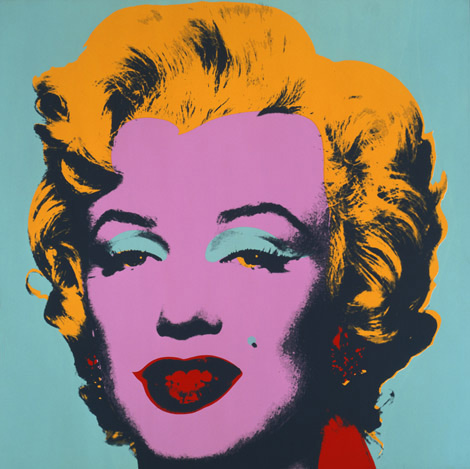
\includegraphics[width=0.68\textwidth]{art-marilyn}
    \caption{Pop-art slika umetnika Andy Warhol}
    \label{fig:art-marilyn}
\end{figure}


\chapter{Princip delovanja instalacije}
``15 sekund slave'' je interaktivna umetniška instalacija, ki obraz naključno
izbranega obiskovalca galerije povzdigne v umetniški objekt za petnajst
sekund. Instalacija je bila navdahnjena s slavnim citatom Andyja Warhola: ``V
prihodnosti bodo vsi ljudje doživeli svojih petnajst minut
slave''\footnote{Originalno v angleščini: \textit{``In the future everybody
will be world-famous for fifteen minutes''}\cite{andyExhibition}.} kot tudi z
njegovim načinom predelave obrazov v slogu pop-art~\cite{solina200215}.

Če pogledamo sliko~\ref{fig:15sec} vidimo le ``mojstrovino'', uokvirjeno v
dragocen okvir. V resnici pa se za to podobo skriva še mnogo več.

\begin{figure}
    \centering
    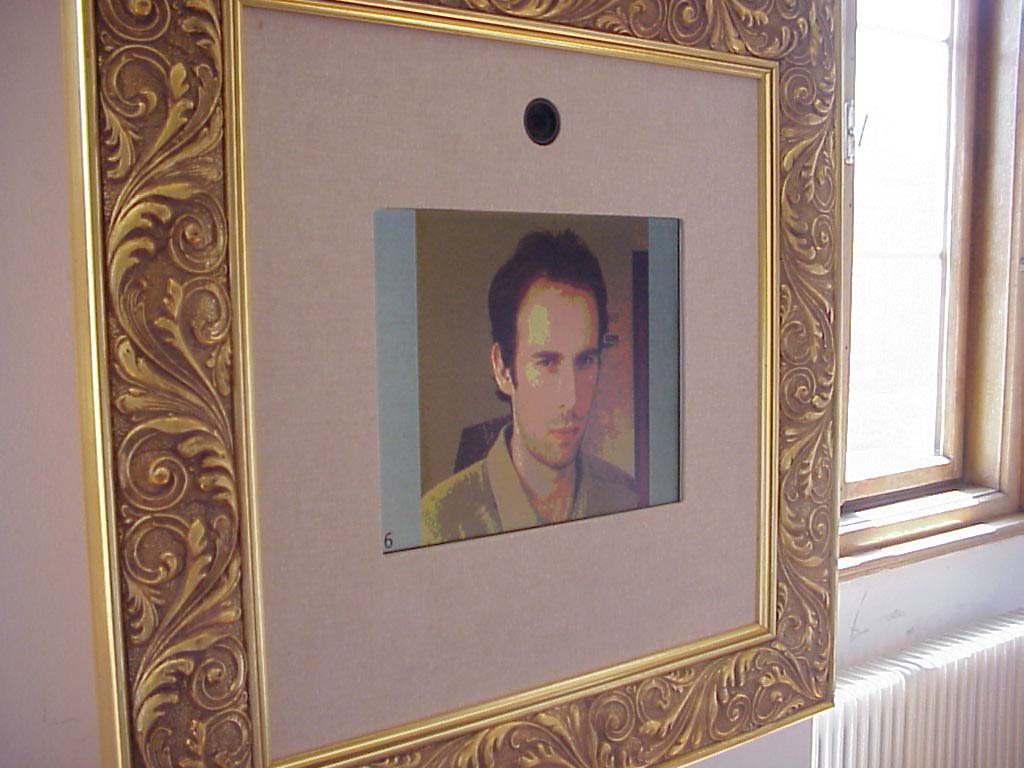
\includegraphics[width=0.7\textwidth]{15sec}
    \caption{Prikaz delovanja instalacije}
    \label{fig:15sec}
\end{figure}

Nad sliko obraza vidimo črno luknjo, to je prostor za digitalni fotoaparat, ki
enkrat na vsakih petnajst sekund fotografira okolico in fotografijo pošlje
računalniku, ki je skrit v ozadju. Fotoaparat ima širokokoten objektiv, da
lahko zajame čim širšo okolico.

Vsako novo fotografijo nato pošljemo računalniku, ki izvede algoritem za
iskanje obrazov. Če je le teh več, enega izberemo po principu naključnega
izbora. Ta obraz izrežemo iz fotografije in ga pošljemo kot vhod
naslednjemu algoritmu.

Izbran obraz se obdela z enim izmed v naprej določenih barvnih filtrov. Ti
filtri so sestavljeni iz različnih barvnih transformacij, da preoblikujejo
fotografijo v slogu pop-art. Pop-art filtri so bolj podrobno opisani v
poglavju~\ref{ch:obdelavaSlik}, primer pop-art transformacije pa lahko vidimo
tudi na sliki~\ref{fig:lena_filter_5}.

Slika obraza v slogu pop-art je končni rezultat, ki je prikazan takoj, ko
prejšnjemu obrazu poteče njegovih petnajst sekund. In kako je prikazan? Pod
luknjo za fotoaparat je izrezan še večji pravokotnik, za katerim se skriva
računalniški zaslon LCD, ki je povezan z računalnikom, ki je opravil
transformacijo fotografije.

Ta postopek se ponavlja v neskončnost, posebnost instalacije pa je, da se vse
dogaja v živo. Če bo torej nekdo dovolj dolgo gledal v okvir, ima veliko
možnosti, da bo kmalu zagledal samega sebe kot ``mojstrovino'' v galeriji.




\chapter{Prvotna izvedba: 15 sekund slave}
Kot že omenjeno, je prvotna instalacija nastala pred več kot 10 leti, zato je
posodobitev več kot zaželena.

\begin{figure}[!ht]
    \centering
    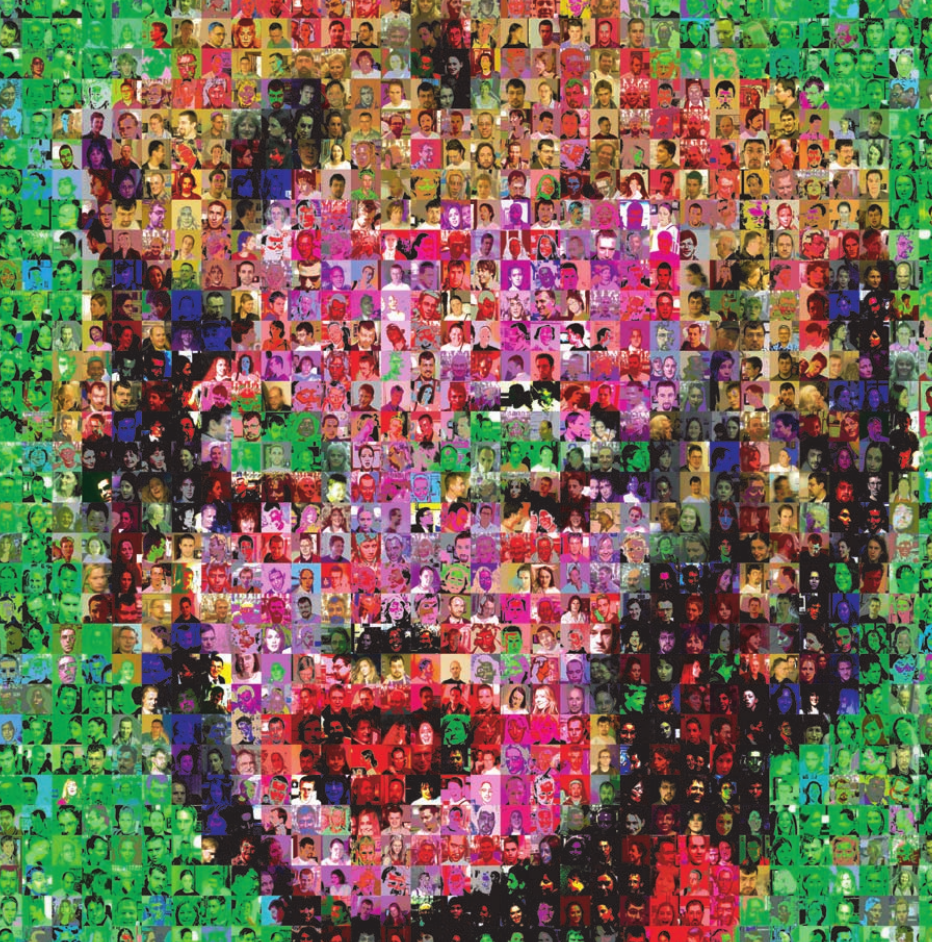
\includegraphics[width=0.68\textwidth]{15sec-marilyn}
    \caption{15 sekund slave slike umetnika Andy Warhol}
    \label{fig:15sec-marilyn}
\end{figure}

\section{Strojna in programska oprema}
Prva razstavljena različica je imela bogato okrašen lesen okvir, ki pa ni bil
prenosen. Za tem okvirjem se je skrival računalniški zaslon LCD, velikosti 17
palcev, malo nad tem zaslonom pa je bil fiksiran digitalni fotoaparat Olympus
C3020 ZOOM (objektiv tipa 32–96mm, maksimalna resolucija je 2048x1536).

Ob selitvi instalacije se je pripetila prva nadgradnja. Lesen okvir se je
zamenjal za malo manj kompaktnega in prenosljivega. V tem času je tudi
tehnologija naredila korak naprej. Naprave so postajale vse manjše in
močnejše. 17 palčni računalniški zaslon je nadomestil 19 palčni, kljub temu pa
se sama velikost naprave ni povečala. Zamenjal se je tudi digitalni
fotoaparat. Zaradi programske opreme je bil najprimernejši kar Olympus, in ker
je bil še vedno željen široki kot objektiva, je to napravo nadomestil Olympus
C40 ZOOM (objektiv tipa 35-98mm, maksimalna resolucija 2272x1704).

Omenjeno je bilo, da je bil Olympus primeren zaradi programske opreme. Ta
digitalni fotoaparat je omogočal upravljanje same naprave programsko preko
računalnika. Orodje SDK omogoča nastavljanje ISO, odprtosti zaslonke, hitrosti
slikanja, fokusa, možnosti zajemanja slike,... S tem je omogočeno avtomatsko
zajemanje nove slike vsakih petnajst sekund.


\chapter{Ohranjanje digitalne umetnosti}
Ohranjanje digitalne umetnosti je zelo pomembna vrednota v svetu
umetnosti~\cite{ZKM}. Navezuje se na umetnost, ki je sicer že v digitalni
obliki, a mora zaradi zelo hitrega razvoja tehnologije vseeno ostati v koraku
s časom. Novejša tehnologija nam omogoča močnejše in hitrejše naprave, manjšo
porabo energije, bolj točne algoritme in še veliko drugih pomembnih izboljšav.
Vendar pa umetnost ni le tehnologija, umetnost je nekaj, kar se ohranja skozi
leta, desetletja, stoletja in še dlje.

Pri digitalni umetnosti se pojavi kar nekaj težav, ki jih pri ohranjanju
običajnih umetniških produktov ni. Če nismo v koraku s časom, je možnost, da
strojna oprema, ki jo potrebujemo za instalacijo, ni več dobavljiva na trgu,
ali pa je že dovolj stara, da ima zgodovinsko vrednost. Nova strojna oprema
doprinese še programske posodobitve, nove principe, standarde in različna
delovanja. Zato je res pomembno, da sledimo razvoju, obenem pa se še vedno
trudimo, da zunanji obiskovalec kljub novi tehnologiji misli, da je to ista,
prvotna instalacija.

In ko že ravno govorimo o novi strojni in programski opremi, omenimo še drugo
težavo. Zaposleni v muzejih in galerijah običajno niso izobraženi za
vzdrževanje digitalne umetnosti, saj ti ljudje načeloma niso strokovnjaki
računalniške stroke. Posledično so možne težave pri rokovanju s tako umetnino,
zato bi bilo priporočljivo, če bi bila instalacija podrobno dokumentirana, in
bi bilo tako pojasnjeno kako jo postaviti, kako jo vzdrževati in kaj storiti v
primeru težav.

Generalno gledano obstajata dve splošni strategiji za ohranjanje digitalne
umetnosti:
\begin{itemize}
\item
Ohraniti želimo vso strojno in programsko
opremo dokler je  to le mogoče. S tem zagotovimo, da je uporabniška izkušnja
ves čas ista. Tukaj bi se večina lahko vprašala, zakaj ne bi strojne opreme s
časom nadgrajevali. Vzemimo primer računalniški zaslon. Res je, tehnologija
LCD je zelo napredovala, slika je v primerjavi s sliko na zaslonih s katodno
cevjo kar nekajkrat bolj ostra in čista. Vendar pa ravno ta ostrina lahko
popolnoma spremeni končni produkt, saj je bil morda nekdo nad umetnino
navdušen ravno zaradi teh zabrisanih robov, ki so ji dajali nekoliko starinski
pridih.

\item
Druga strategija je, da nadgradimo strojno in programsko opremo. Pri tem
moramo biti zelo pazljivi, da uporabnik še vedno dobi tisto, kar je dobil pred
nadgradnjo. Umetniška instalacija mora ostati kar se da podobna prejšnji,
vključno z vsemi funkcionalnostmi. Vendar pa se pogosto zgodi, da avtor skozi
čas pridobi nove ideje za posodobitve, velikokrat gre tako za nekaj, kar prej
s staro tehnologijo sploh še ni bilo mogoče. Lep primer take ideje je
integracija s socialnimi omrežji.
\end{itemize}


\chapter{Nadgradnja: Naprava in pripomočki}
Kot prvo nadgradnjo, ki smo si jo zamislili, je čim bolj učinkovito zmanjšati
porabljen prostor za instalacijo in s tem olajšati njeno prenosljivost in
povečati enostavnost postavitve.

Prvotna instalacija potrebuje osebni ali prenosni računalnik, zaslon LCD,
digitalni fotoaparat, mrežno opremo in dostop do interneta.

Kot najboljša zamenjava se je izkazala naprava ``pametni telefon'', saj ima
vse prej naštete naprave združene v eno. Ima vgrajeno kamero, ki služi kot
fotoaparat, dostop do interneta preko kartice SIM ter operacijski sistem, ki
omogoča izdelavo programske opreme s katero lahko dostopamo do prej naštetih
funkcij.

Pametni telefoni dražje stopnje omogočajo tudi, da lahko sliko v živo
predvajamo na večjem ekranu. Zato smo se odločili, da kot testno napravo
vzamemo pametni telefon Samsung Galaxy S5.

\section{Testna naprava: Samsung Galaxy S5}

\begin{figure}[!ht]
    \centering
    \begin{subfigure}[b]{0.4\textwidth}
        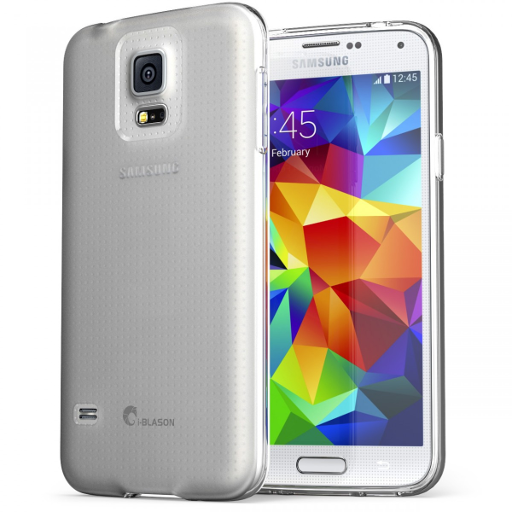
\includegraphics[width=\textwidth]{sgs5full}
    \end{subfigure}
    \begin{subfigure}[b]{0.4\textwidth}
        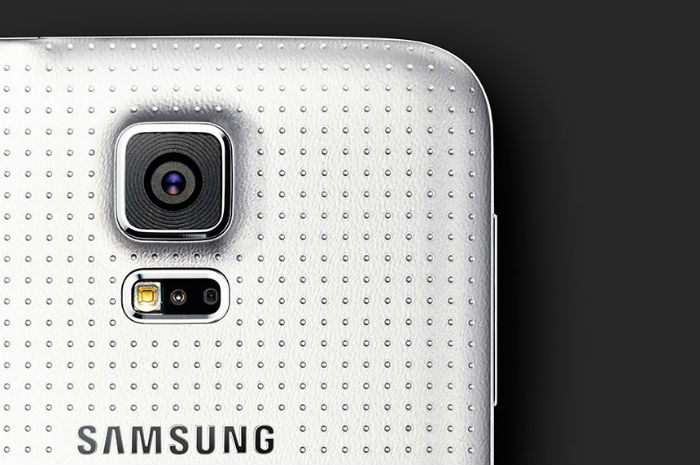
\includegraphics[width=\textwidth]{sgs5camera}
        \caption{Kamera z bliskavico}
    \end{subfigure}
    \caption{Testna naprava: Samsung Galaxy S5}
    \label{fig:sgs5}
\end{figure}

Samsung Galaxy S5 je pametni telefon, narejen v podjetju Samsung. Deluje na
operacijskem sistem Android verzije 4.4.4, imenovanem tudi Android Kitkat.
Trenutno najnovejši obstoječi operacijski sistem Androida je verzija 5.0,
poimenovan Lizika (\textit{angl. Lolipop}).

Samsnug Galaxy S5 se ponaša s štiri-jedrnim procesorjem 2.5GHz Krait 400 na
čipu Qualcomm MSM8974AC Snapdragon 801. Ta procesor je dovolj zmogljiv za
preračunavanje vseh filtrov v zadovoljivem času.

Grafična enota, Adreno 330, omogoča možnost prikazovanja v resoluciji
1080~x~1920 pikslov. Ena izmed pomembnih lastnosti je tudi možnost povezave
zunanje naprave preko priključka HDMI.

Tudi kamera je  izjemno kvalitetna, je namreč tipa 1/2.6''. Svetlobno tipalo
ima šestnajst mega pikslov, kar lahko naredi sliko v velikosti 5312~x~2988
pikslov. Velikost in obliko kamere lahko vidimo kot majhen črn kvadrat, viden
na desni sliki~\ref{fig:sgs5}.

Pomembna lastnost je tudi operacijski sistem Android, za katerega je v
programskem jeziku Java mogoče napisati programsko opremo imenovano
aplikacija. Vse kar za to potrebujemo, je Android SDK in prevajalnik Java.


\section{Android}
Android je odprtokodni sistem za pametne telefone, ki ga je leta 2007 izdelal
Open Handset Alliance pod vodstvom podjetja Google. Projekt se imenuje
AOSP~\footnote{Celotno ime je Android Open Source Project} in se še danes zelo
hitro razvija.

Temelji na jedru Linux, najbolj bistven del arhitekture pa je navidezni stroj
(\textit{angl. virtual machine}). Bolj podrobna zgradba sistema je prikazana
na sliki~\ref{picAndroid}. Navidezni stroj, imenovan Dalvik virtual machine,
vsebuje prevajalnik JIT, ki je zadolžen za zaganjanje že prevedene programske
kode Java. Prevedena koda je zapakirana v datoteke s končnico .apk. Tem
datotekam pravimo aplikacije, izdelane za sistem Android.

\begin{figure}
    \centering
    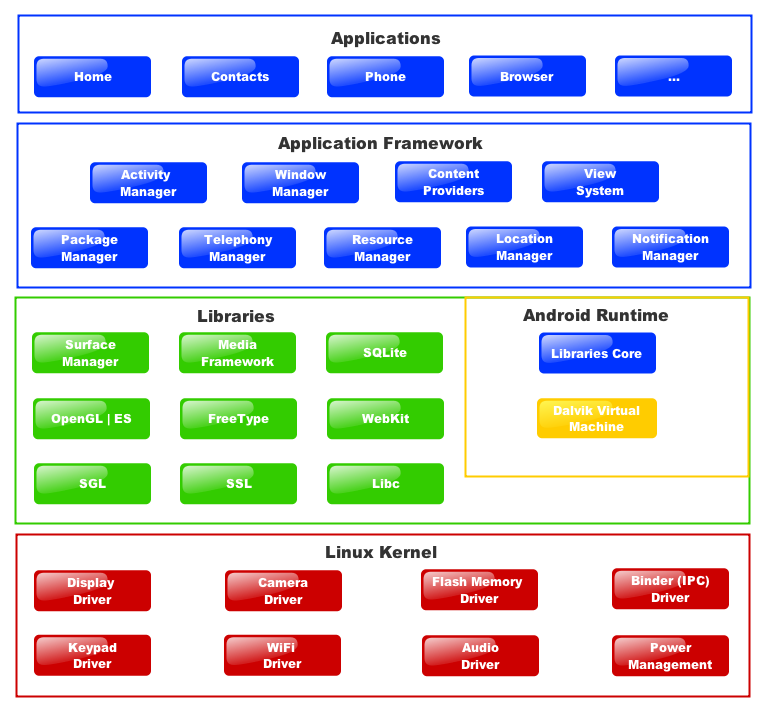
\includegraphics[width=\textwidth]{android}
    \caption{Struktura operacijskega sistema Android~\cite{wiki:Android}}
    \label{picAndroid}
\end{figure}

Za izdelavo aplikacije Android potrebujemo znanje programskega jezika Java,
Android SDK, ki je brezplačno na voljo na uradni spletni
strani\footnote{Uradna spletna stran je dostopna na {\tt
http://developer.android.com/}}. Priporočljivo je tudi branje dokumentacije
SDK, ki je na voljo na spletu\footnote{Dokumentacija SDK je dostopna na {\tt
http://developer.android.com/sdk/}}. Dokumentacija je napisana zelo
razumljivo, tako da se lahko znajdejo tudi začetniki. S pomočjo Android SDK na
koncu nastane datoteka .apk.

\chapter{Nadgradnja: Zaznavanje obrazov}
Operacijski sistem Android nam preko vmesnika JNI omogoča vključevanje
programskega jezika C. Posledično lahko uporabljamo splošne knjižnice in
programska ogrodja (\textit{angl. framework}).

Ker smo v naši nadgradnji želeli, da bi se obrazi zaznavali v realnem času,
smo se odločili za uporabo programskega ogrodja OpenCV.

\section{Zaznavanje obrazov z uporabo OpenCV}
OpenCV je programsko ogrodje, ki nam omogoča izvedbo raznih operacij,
izvedenih nad slikami. Napisana je v programskem jeziku C, za potrebe
operacijskega sistema Android pa so napisani tudi povezovalni Java razredi
(\textit{angl. class}), ki nam omogočajo uporabo OpenCV operacij kar preko
programskega jezika Java.

Najpomembnejša funkcionalnost programskega ogrodja OpenCV za nas je bila
implementacija zaznavanja obrazov. Ta uporablja algoritem kaskadnega
klasificiranja (\textit{angl. cascade classifier}), ki nam omogoča
klasifikacijo različnih lastnosti.

Lastnosti so zapisane v datoteki XML. Ta datoteka vsebuje več sto ali tisoč
različnih lastnosti, ki opisujejo določen predmet, kar v našem primeru pomeni
obliko obraza.

Obstaja več različnih tipov, preko katerih so te lastnosti opisane. Za
zaznavanje obrazov sta najpomembnejša tipa ``HAAR'' in ``LBP''. Tipa se
razlikujeta po točnosti in hitrosti.

``HAAR'' opisi so procesorsko bolj potratni in potrebujejo relativno veliko
časa za prepoznavo obraza, vendar pa je zato veliko manj napačnih detekcij
(\textit{angl. false positive}).

``LBP'' pa je, čeprav z nekaj več napakami pri klasifikaciji kot HAAR'', za
naše potrebe še vedno dovolj točen. Njegova glavna prednost pred prej
opisanim je  njegova hitrost, kar je pri detekciji obrazov v živo zelo
pomembno, če želimo doseči zadovoljstvo uporabnika.

Ker so si obrazi med seboj zelo različni, je nemogoče, da bi bil najden prav
vsak obraz, vseeno pa želimo, da je število zgrešenih obrazov čim manjše.
Vendar pa zgrešen obraz ni največja težava, saj uporabnik tega najbrž ne bi
opazil. Veliko bolj neprijetna težava je, če najdemo obraz tam, kjer ga ni, na
primer nek predmet v okolici, ki ga zaznamo in obdelamo kot obraz.

Testirali smo oba tipa z različnimi tipi lastnosti. Pri tem smo uporabili le
lastnosti, ki opisujejo sprednji del obraza. Vendar pa se je pri uporabi
``LBP'' opisov še vedno pokazalo preveč lažnih obrazov. Zato smo se odločili
za uporabo lastnosti tipa ``HAAR''. Veliko bolj se nam zdi namreč pomembno, da
ima petnajst sekund slave obraz uporabnika, in ne kakšen predmet v okolici, pa
čeprav je za to potrebno nekoliko več časa.

Vendar pa tudi tipi ``HAAR'' opisi obrazov niso vedno dosegli našega
pričakovanja. Zato smo se odločili, da naredimo dvojno klasifikacijo.

Najprej smo klasificirali z lastnostmi sprednjega dela obraza, opisanimi v
datoteki \textit{harrcascade\_frontalface\_default.xml}~\ref{lst:haar_frontal_face},
s katerimi smo dobili rezultate obrazov. Ker se je že za samo klasifikacijo
obraza porabilo kar nekaj časa, smo se odločili, da iskanje prekinemo takoj po
najdenem prvem obrazu, ki je velik vsaj eno desetino celotne slike.

\pagebreak % TODO: zbriši
\begin{lstlisting}[label=lst:haar_frontal_face, caption=Izsek iz datoteke harrcascade\_frontalface\_default.xml]
<maxWeakCount>9</maxWeakCount>
<stageThreshold>-5.0425500869750977e+00</stageThreshold>
<weakClassifiers>
  <_>
    <internalNodes>
      0 -1 0 -3.1511999666690826e-02
    </internalNodes>
    <leafValues>
      2.0875380039215088e+00 -2.2172100543975830e+00
    </leafValues>
  </_>
  <_>
    <internalNodes>
      0 -1 1 1.2396000325679779e-02
    </internalNodes>
    <leafValues>
      -1.8633940219879150e+00 1.3272049427032471e+00
    </leafValues>
  </_>
  ...
\end{lstlisting}

Kandidata obraza smo testirali še s klasifikacijo očesa. Vsak obraz ima dve
očesi. Zavedali smo se, da v primeru očal tega ne bomo našli, vendar pa se je
izkazalo da težave nastopijo le pri zasenčenih očalih. Za to klasifikacijo smo
uporabili lastnosti, zapisane v datoteki \textit{harrcascade\_eye.xml}~\ref{lst:haar_eye}.
V primeru, da smo našli točno dva rezultata, smo vrnili prejšnji rezultat,
v nasprotnem primeru pa javili, da obraz ni najden.

\begin{lstlisting}[label=lst:haar_eye, caption=Izsek iz datoteke harrcascade\_eye.xml]
<maxWeakCount>6</maxWeakCount>
<stageThreshold>-1.4562760591506958e+00</stageThreshold>
<weakClassifiers>
  <_>
    <internalNodes>
      0 -1 0 1.2963959574699402e-01
    </internalNodes>
    <leafValues>
      -7.7304208278656006e-01 6.8350148200988770e-01
    </leafValues>
  </_>
  <_>
    <internalNodes>
      0 -1 1 -4.6326808631420135e-02
    </internalNodes>
    <leafValues>
      5.7352751493453979e-01 -4.9097689986228943e-01
    </leafValues>
  </_>
  ...
\end{lstlisting}

S temi nastavitvami in omejitvami smo dosegli pričakovane rezultate. Polje z
najdenim rezultatom smo povečali še za približno eno tretjino, tako da je
končni produkt zajemal nekoliko večji predel osnovne slike in je bil kvadratne
oblike. Zakaj ravno eno tretjino? Iskali smo prednji del obraza in ga tudi
našli. Vendar si v okvirju želimo videti sliko celotne glave in ne samo
obraza. Povečava polja za eno tretjino se je izkazala kot ravno pravšnja za
večino testiranih primerov.

\begin{figure}[!ht]
    \centering
    \begin{subfigure}[b]{0.3\textwidth}
        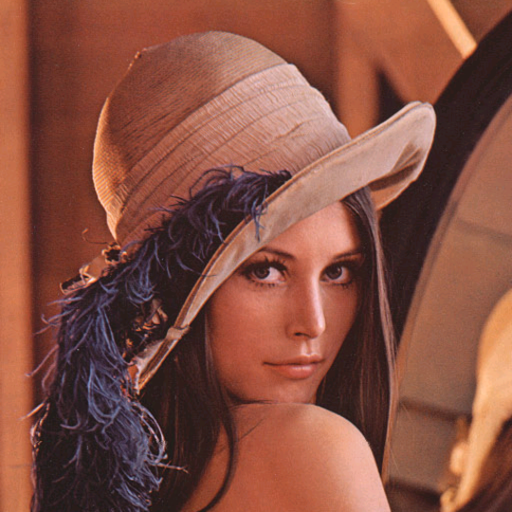
\includegraphics[width=\textwidth]{lena}
        \caption{Original}
    \end{subfigure}
    \begin{subfigure}[b]{0.3\textwidth}
        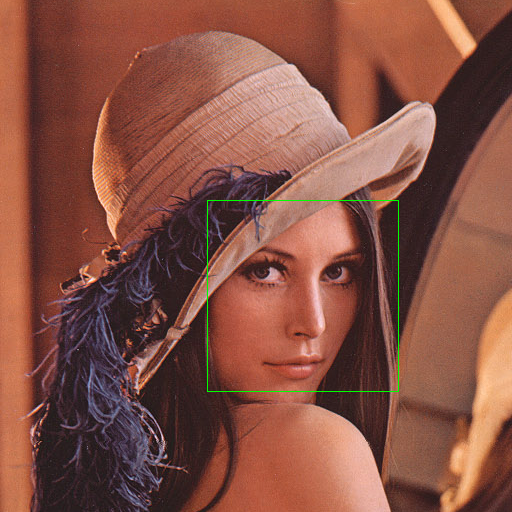
\includegraphics[width=\textwidth]{lena_opencv_face}
        \caption{Zaznavanje obraza}
        \label{fig:lena_opencv_face}
    \end{subfigure}
    \begin{subfigure}[b]{0.3\textwidth}
        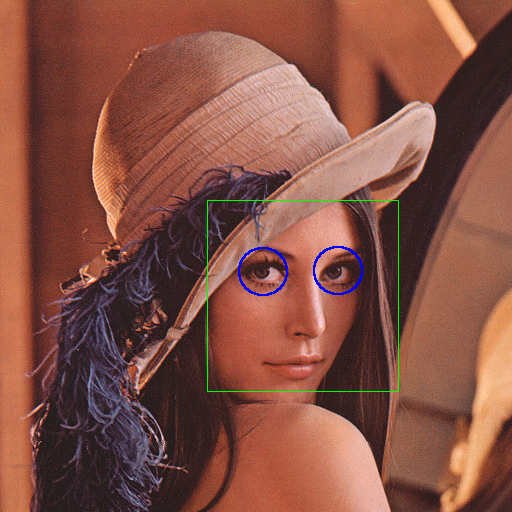
\includegraphics[width=\textwidth]{lena_opencv_face_eye}
        \caption{Zaznavanje oči}
        \label{fig:lena_opencv_face_eye}
    \end{subfigure}
    \caption{Prikaz zaznavanja obraza in oči s programskim ogrodjem OpenCV}
\end{figure}

Detekcija obrazov s programskim ogrodjem OpenCV je le ena izmed možnosti, ki
smo si jih podrobneje ogledali. Kot prva implementacija je bila izbrana zaradi
velike kontrole nad vsakim korakom, kot so: detekcija
obraza~\ref{fig:lena_opencv_face}, določitev regije kje je potrebno iskati,
detekcija oči v določeni regiji~\ref{fig:lena_opencv_face_eye} in še bi lahko
naštevali.

Kljub zadovoljivim rezultatom iskanja obrazov se je izkazalo, da slike
velikokrat niso ostre. Prej smo omenili, da imamo veliko kontrolo nad
različnimi algoritmi za detekcijo, kar pa ne vključuje uporabe kamere, ki je v
pametnem telefonu. OpenCV uporablja sliko iz kamere tako kot je, brez
predhodne izostritve. Povedano z drugimi besedami, uporablja jo kot kamero in
ne kot digitalni fotoaparat.


\section{Zaznavanje obrazov z uporabo Android SDK}
Android SDK deluje povsem drugače kot OpenCV. Ne omogoča nobene kontrole in
parametrov, možna je uporaba le v naprej določenega algoritma.

Ta algoritem bazira na algoritmu NV1-NORM~\cite{nevenFaceRecognition}, ki ga
je izdelalo podjetje Neven Vision~\ref{fig:neven_vision}. Leta 2006 je Neven
Vision postalo last podjetja Google in od takrat se uporablja za zaznavo
obrazov v mnogih programih, ki jih je izdelalo podjetje Google. Lep  primer je
program za prikaz slik Google Picassa.

\begin{figure}[!ht]
    \centering
    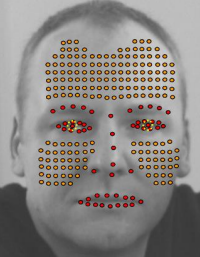
\includegraphics[width=0.3\textwidth]{neven_vision}
    \caption{Vizualizacija zaznavanja obraza, Neven Vision}
    \label{fig:neven_vision}
\end{figure}

Natančnejša implementacija algoritma za zaznavo obraza je zaprto-kodna. Če si
ogledamo dokumentacijo Android SDK-ja, je opisan samo primer uporabe:
\pagebreak % TODO: zbriši
\begin{lstlisting}[caption="Primer uporabe zaznavanja obraza z orodjem Android SDK"]
FaceDetector fc = new FaceDetector(
    sirina_slike,
    visina_slike,
    maksimalno_stevilo_obrazov
).findFaces(slika, obrazi);
\end{lstlisting}

Vendar pa kljub zaprtosti in nezmožnosti prilagajanja detektorja prinaša zelo
dobre rezultate. Ker so vse funkcije že vključeno v operacijski sistem, tudi
ne potrebujemo dodatnih programskih ogrodij. S tem smo si prihranili kar nekaj
časa in prostora.

Rezultat zaznavanja obraza pa tokrat ni obraz sam. Kot rezultat dobimo
razdaljo med očmi, rotacijo obraza ter točko med očmi. Na podlagi teh podatkov
lahko določimo regijo, na kateri je obraz na sliki.

Testirali smo razlike med rezultati obeh algoritmov in se na koncu odločili za
uporabo Android SDK. Kot že opisano, poleg dobrih rezultatov pridobimo še na
velikosti končne aplikacije in kompleksnosti celotnega programa.


\chapter{Nadgradnja: Obdelava slik}
\label{ch:obdelavaSlik}
Instalacija ``15 sekund slave'' vsebuje 17 različnih
filtrov~\cite[Poglavje~5]{thesisSamoJuvan} za obdelavo prejetih slik v
pop-art slike. Filtri so bili izdelani s pomočjo grafičnega programa GIMP.


\section{GIMP}
GIMP je odprto-kodno programsko orodje za obdelavo slik.


\subsection{Zgodovina}
Začetek projekta sega v leto 1995, kjer se je vse skupaj začelo kot
semestrski projekt na Univerzi Kalifornije, Berkeley. Avtorja Spencer Kimball
in Peter Mattis sta projekt poimenovala \textit{angl. General Image
Manipulation Program}, čez nekaj časa pa sta si premislila in Richarda
Stallmana, ki je ravno takrat obiskal univerzo, prosila, če lahko spremenita
besedo ``General'' v ``GNU''. Od takrat naprej se program imenuje
\textit{angl. GNU Image Manipulation Program} ali na kratko še vedno
GIMP~\cite{wiki:GIMP}.


\section{Izbira filtrov}
Že naša prvotna izbira filtrov je izhajala iz programskega orodja za predelavo
slik GIMP. Zaradi lažjega dela se je najprej, s pomočjo grafičnega vmesnika,
izbralo zaporedje različnih filtrov in njihove parametre.  Izbrani so bili
naslednji filtri:
\begin{itemize}
    \item \textbf{uravnovešanje barv} \textit{angl. color balance} \hfill \\
        Prekrije celotno sliko z barvo v izbranem odtenku.
    \item \textbf{posteriziranje} \textit{angl. posterize} \hfill \\
        Zmanjšuje število barv na sliki.
    \item \textbf{uravnovešanje barv v HSL prostoru} \textit{angl. hue saturation balance} \hfill \\
        Spreminja odtenke barv, svetlost in intenzivnost na sliki.
\end{itemize}


\section{Implementacija filtrov}
Ker je GIMP odprto-koden smo imeli tudi dostop do implementacije filtrov.
Implementacije filtrov so napisane v programskem jeziku C. Na prvi pogled kot
nalašč za enostaven prenos na Android platformo preko JNI. Vendar pa so se
pokazale težave, saj so bili filtri močno povezani z GIMP objekti in nekoliko
bolj kompleksni, kot bi bilo potrebno za naš projekt. Zato smo se odločili, da
filtre ponovno implementiramo, ter zavržemo vse funkcionalnosti, ki za nas niso
pomembne. Naredili smo tri različne implementacije in jih med seboj primerjali.

Prva implementacija je napisana v programskem jeziku java. Izkazala se je za
zelo počasno. Orodje za sproščanje pomnilnika GC \textit{(angl. garbage
collector)} se je klicalo prepogosto, kar je posledično porabilo več kot nekaj
sekund za filter. Tega si nismo mogli privoščiti, zato smo iskali alternative.

Naslednja implementacija je napisana s pomočjo grafične kartice in sicer z
orodjem OPENGL ES, verzije 2.0. Čas porabe pri izvajanju se je občutno
zmanjšal. Ko so bile teksture zapisane na grafični kartici, so se filtri
izvajali v manj kot sekundi. Ta rešitev je bila že dovolj dobra, vendar pa se
nam je zdelo, da je uporaba grafične kartice za tako lahke operacije potrata
energije.

Čeprav so bili rezultati že dovolj dobri, smo se odločili še za implementacijo
v programskem jeziku C. Rezultati so pokazali, da je ta rešitev nekoliko
počasnejša kot prejšnja, vendar pa za to nismo potrebovali grafične kartice na
telefonu. Porabljen čas je bil manj kot sekundo za filter.

\subsection{HSL barvni prostor}
\label{sec:hsl}

\begin{align}
R, G, B &\in [0,255] \nonumber \\
Cmax &= max(R, G, B) \\
Cmin &= min(R, G, B) \\
\Delta &= (Cmax - Cmin)
\end{align}

\begin{equation}
L = (max + min) / 2 \label{eq:hsl_l}
\end{equation}

\begin{equation}
S =
\begin{cases}
    0 \text{,}& \Delta = 0 \\
    255 * \Delta / (Cmax + Cmin) \text{,}& L < 128 \\
    255 * \Delta / (511 - Cmax - Cmin) \text{,}& \text{ostalo}
\end{cases}
\end{equation}

\begin{equation}
H' =
\begin{cases}
    0 \text{,}& \Delta = 0 \\
    0 + 42.5 * (G - B) / \Delta \text{,}& R = Cmax \\
    85 + 42.5 * (B - R) / \Delta \text{,}& G = Cmax \\
    170 + 42.5 * (R - G) / \Delta \text{,}& B = Cmax
\end{cases}
\end{equation}

\begin{equation}
H =
\begin{cases}
    H' + 255 \text{,}& H' < 0 \\
    H' - 255 \text{,}& H' > 255 \\
    H' \text{,}& \text{ostalo}
\end{cases}
\end{equation}

\begin{lstlisting}[caption=algoritem]
Cmax = max(R, G, B)

\end{lstlisting}

\subsection{Uravnovešanje barv}

\begin{equation}
clamp_{min}^{max}(x) =
\begin{cases}
    min \text{,}& x < min \\
    max \text{,}& x > max \\
    x \text{,}& \text{ostalo}
\end{cases}
\end{equation}

\begin{align}
shadows(x) &= clamp_{0}^{1}(\frac{117 - x}{64}) * 1.785 \\
color\_balance(x, x') &= clamp_{0}^{255}(x + x' * shadows(x)) \label{eq:color_balance}
\end{align}

Uravnovešanje barv se računa v barvnem prostoru RGB. Računamo jo za vsako
barvo posebej, in sicer z enačbo~\eqref{eq:color_balance}, kjer je $x$ enak
originalni barvi, $x'$ pa barvi, s katero želimo uravnovesiti originalno barvo
$x$. $x$ in $x'$ sta pozitivni celi števili med 0 in 255.

Po izračunanih vrednostih dane rezultate iz RGB prostora prenesemo v HSL
prostor s pomočjo enačb, napisnih v poglavju~\ref{sec:hsl}. Tako dobimo $H$,
$S$ in $L$. Iz originalnih vrednosti, to je vrednost barve na sliki,
izračunamo $L$~\ref{eq:hsl_l} in ga nadomestimo s prejšnjim, zato da ohranimo
podobno svetlost. $H$, $S$ in novo pridobljeni $L$ prenesemo nazaj v RGB
prostor.

\subsection{Posteriziranje}

\begin{equation}
luts(x, levels) = 255 * \frac{\left \lfloor{\frac{x}{255} * (levels - 1) + 0.5}\right \rfloor}{levels - 1} + 0.5
\end{equation}

Posteriziranje se računa v barvnem prostoru RGB...

\subsection{Uravnovešanje barv v HSL prostoru}

\begin{align}
htv(x, x') &= x + 255 * \frac{x'}{360} \nonumber \\
hue\_transfer(x, x') &=
\begin{cases}
    htv(x, x') + 255 \text{,}& htv(x, x') < 0 \\
    htv(x, x') - 255 \text{,}& htv(x, x') > 255 \\
    htv(x, x') \text{,}& \text{ostalo}
\end{cases}
\end{align}

\begin{align}
ltv(x, x') &= clamp_{-255}^{255}(1.27 * x') \nonumber \\
lightness\_transfer(x, x') &=
\begin{cases}
    x * \frac{255 + ltv(x, x')}{255} \text{,}& ltv(x, x') < 0 \\
    x + \frac{(255 - x) * ltv(x, x')}{255} \text{,}& ltv(x, x') \geq 0
\end{cases}
\end{align}

\begin{align}
stv(x, x') &= clamp_{-255}^{255}(2.25 * x') \nonumber \\
saturation\_transfer(x, x') &= clamp_{0}^{255}(x + x * \frac{stv(x, x')}{255})
\end{align}

\subsection{Sestavljanje pop-art filtrov}

\subsubsection*{Filter 1}
Prvi filter je sestavljen iz dveh osnovnih filtrov. Najprej sliko obdelamo s
filtrom ``uravnovešanje barv'' in sicer s parametri $R = 30$, $G = -32$ in
$B = 16$. Rezultat obdelamo še s filtrom ``posteriziranje'' s parametrom
$ST =4$. Rezultat testne slike lahko vidimo na sliki~\ref{fig:lena_filter_1}.

\begin{figure}[!ht]
    \centering
    \begin{subfigure}[b]{0.4\textwidth}
        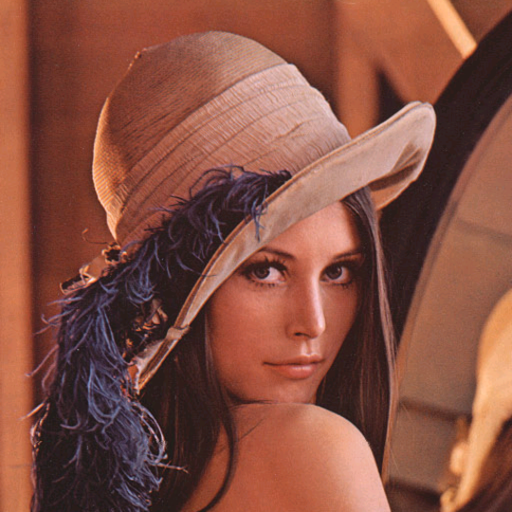
\includegraphics[width=\textwidth]{lena}
        \caption{Original}
    \end{subfigure}
    \begin{subfigure}[b]{0.4\textwidth}
        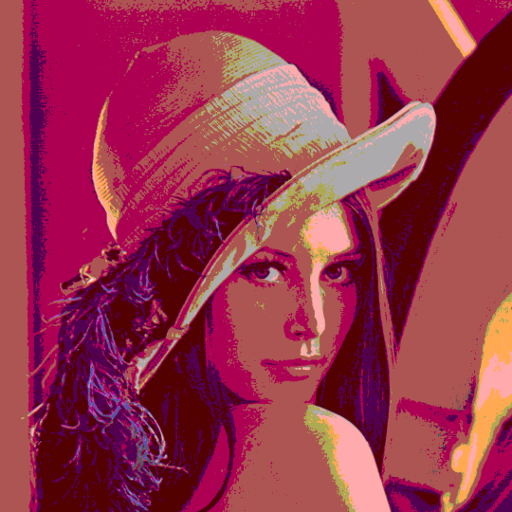
\includegraphics[width=\textwidth]{lena_filter_1}
        \caption{Prvi filter}
    \end{subfigure}
    \caption{Primerjava originalne slike z obdelano sliko}
    \label{fig:lena_filter_1}
\end{figure}


\subsubsection*{Filter 2}
Drugi filter je sestavljen iz dveh osnovnih filtrov. Najprej sliko obdelamo s
filtrom ``uravnovešanje barv'' in sicer s parametri $R = -36$, $G = -37$ in
$B = 39$. Rezultat obdelamo še s filtrom ``posteriziranje'' s parametrom
$ST = 4$. Rezultat testne slike lahko vidimo na sliki~\ref{fig:lena_filter_2}.

\begin{figure}[!ht]
    \centering
    \begin{subfigure}[b]{0.4\textwidth}
        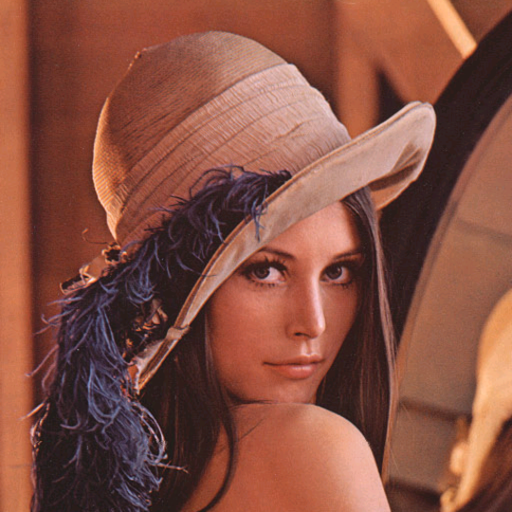
\includegraphics[width=\textwidth]{lena}
        \caption{Original}
    \end{subfigure}
    \begin{subfigure}[b]{0.4\textwidth}
        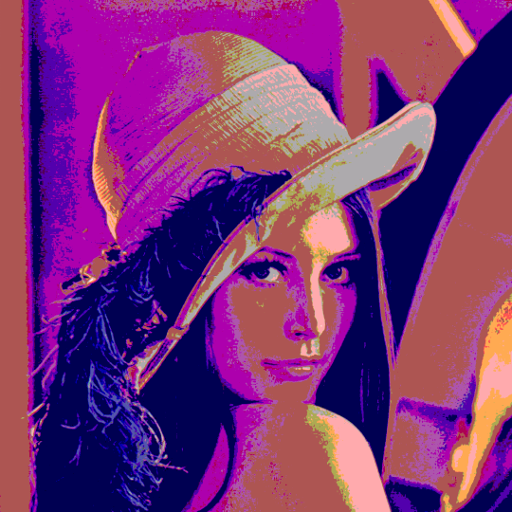
\includegraphics[width=\textwidth]{lena_filter_2}
        \caption{Drugi filter}
    \end{subfigure}
    \caption{Primerjava originalne slike z obdelano sliko}
    \label{fig:lena_filter_2}
\end{figure}


\subsubsection*{Filter 3}
Tretji filter vsebuje le osnovni filter ``posteriziranje'' in sicer s parametrom
$ST = 2$. Rezultat testne slike lahko vidimo na sliki~\ref{fig:lena_filter_3}.

\begin{figure}[!ht]
    \centering
    \begin{subfigure}[b]{0.4\textwidth}
        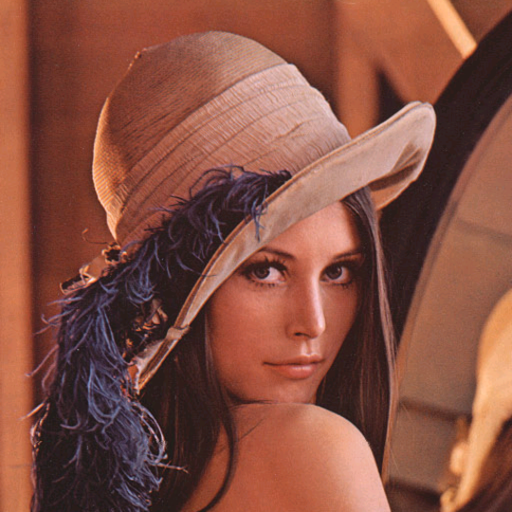
\includegraphics[width=\textwidth]{lena}
        \caption{Original}
    \end{subfigure}
    \begin{subfigure}[b]{0.4\textwidth}
        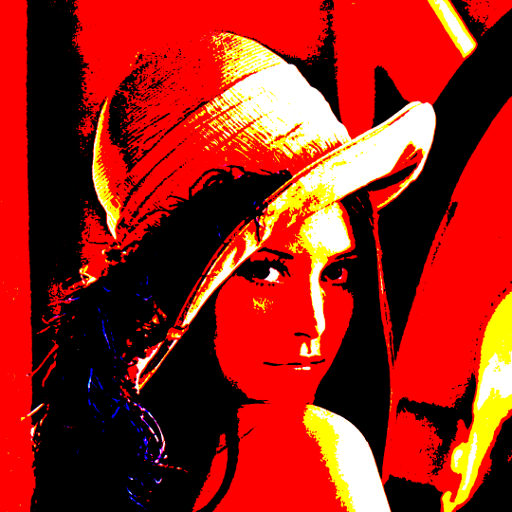
\includegraphics[width=\textwidth]{lena_filter_3}
        \caption{Tretji filter}
    \end{subfigure}
    \caption{Primerjava originalne slike z obdelano sliko}
    \label{fig:lena_filter_3}
\end{figure}


\subsubsection*{Filter 4}
Četrti filter je sestavljen iz dveh osnovnih filtrov. Najprej sliko obdelamo s
filtrom ``uravnovešanje barv'' in sicer s parametri $R = 100$, $G = -100$ in
$B = -100$. Rezultat obdelamo še s filtrom ``posteriziranje'' s parametrom
$ST = 3$. Rezultat testne slike lahko vidimo na sliki~\ref{fig:lena_filter_4}.

\begin{figure}[!ht]
    \centering
    \begin{subfigure}[b]{0.4\textwidth}
        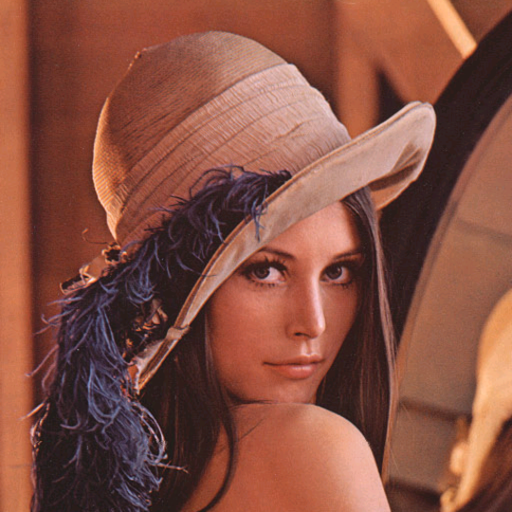
\includegraphics[width=\textwidth]{lena}
        \caption{Original}
    \end{subfigure}
    \begin{subfigure}[b]{0.4\textwidth}
        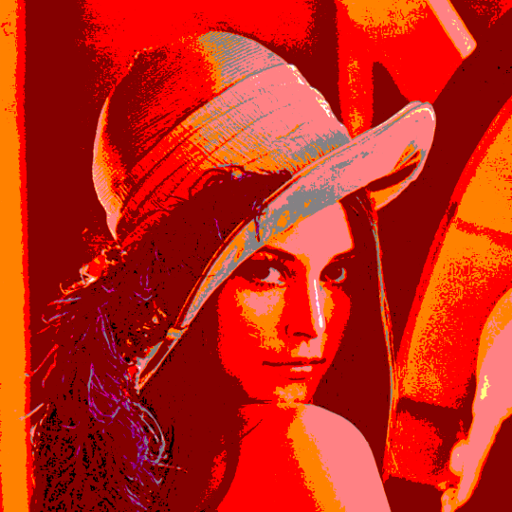
\includegraphics[width=\textwidth]{lena_filter_4}
        \caption{Četrti filter}
    \end{subfigure}
    \caption{Primerjava originalne slike z obdelano sliko}
    \label{fig:lena_filter_4}
\end{figure}


\subsubsection*{Filter 5}
Peti filter je sestavljen iz dveh osnovnih filtrov. Najprej sliko obdelamo s
filtrom ``uravnovešanje barv'' in sicer s parametri $R = -100$, $G = -100$ in
$B = 100$. Rezultat obdelamo še s filtrom ``posteriziranje'' s parametrom
$ST = 3$. Rezultat testne slike lahko vidimo na sliki~\ref{fig:lena_filter_5}.

\begin{figure}[!ht]
    \centering
    \begin{subfigure}[b]{0.4\textwidth}
        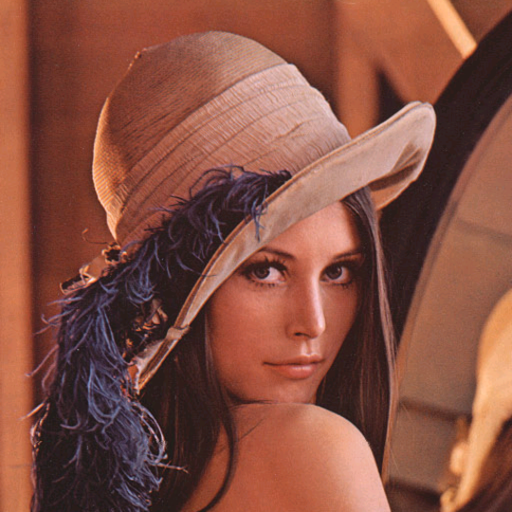
\includegraphics[width=\textwidth]{lena}
        \caption{Original}
    \end{subfigure}
    \begin{subfigure}[b]{0.4\textwidth}
        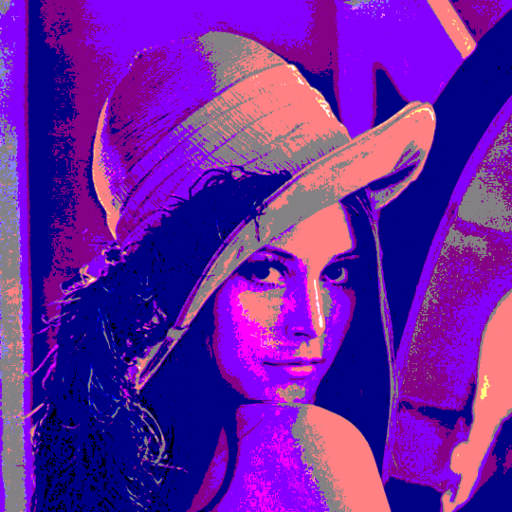
\includegraphics[width=\textwidth]{lena_filter_5}
        \caption{Peti filter}
    \end{subfigure}
    \caption{Primerjava originalne slike z obdelano sliko}
    \label{fig:lena_filter_5}
\end{figure}


\subsubsection*{Filter 6}
Šesti filter je sestavljen iz dveh osnovnih filtrov. Najprej sliko obdelamo s
filtrom ``uravnovešanje barv'' in sicer s parametri $R = -100$, $G = 100$ in
$B = -100$. Rezultat obdelamo še s filtrom ``posteriziranje'' s parametrom
$ST = 3$. Rezultat testne slike lahko vidimo na sliki~\ref{fig:lena_filter_6}.

\begin{figure}[!ht]
    \centering
    \begin{subfigure}[b]{0.4\textwidth}
        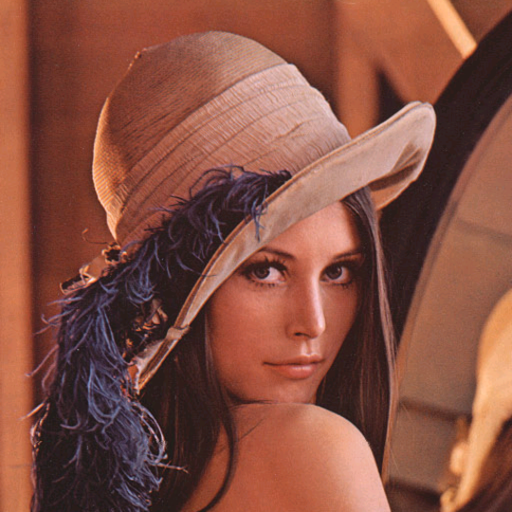
\includegraphics[width=\textwidth]{lena}
        \caption{Original}
    \end{subfigure}
    \begin{subfigure}[b]{0.4\textwidth}
        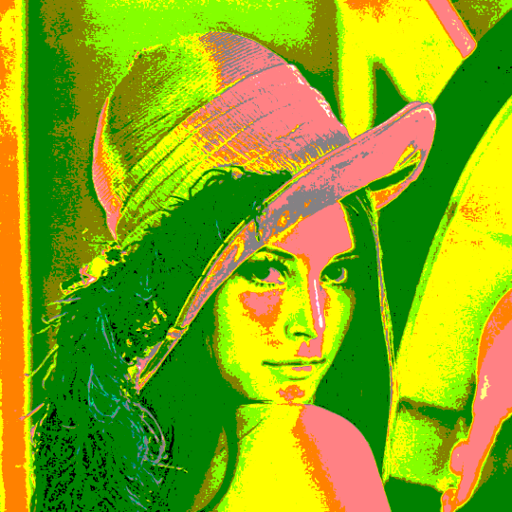
\includegraphics[width=\textwidth]{lena_filter_6}
        \caption{Šesti filter}
    \end{subfigure}
    \caption{Primerjava originalne slike z obdelano sliko}
    \label{fig:lena_filter_6}
\end{figure}


\subsubsection*{Filter 7}
Sedmi filter je sestavljen iz dveh osnovnih filtrov. Najprej sliko obdelamo s
filtrom ``posteriziranje'' in sicer s parametrom $ST = 5$. Rezultat obdelamo
še s filtrom ``uravnovešanje barv v HSL prostoru'' s parametri $H = -41$,
$L = -15$ in $S = 6$. Rezultat testne slike lahko vidimo na
sliki~\ref{fig:lena_filter_7}.

\begin{figure}[!ht]
    \centering
    \begin{subfigure}[b]{0.4\textwidth}
        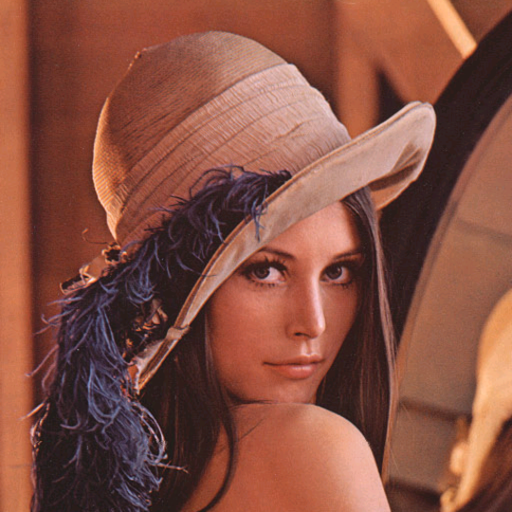
\includegraphics[width=\textwidth]{lena}
        \caption{Original}
    \end{subfigure}
    \begin{subfigure}[b]{0.4\textwidth}
        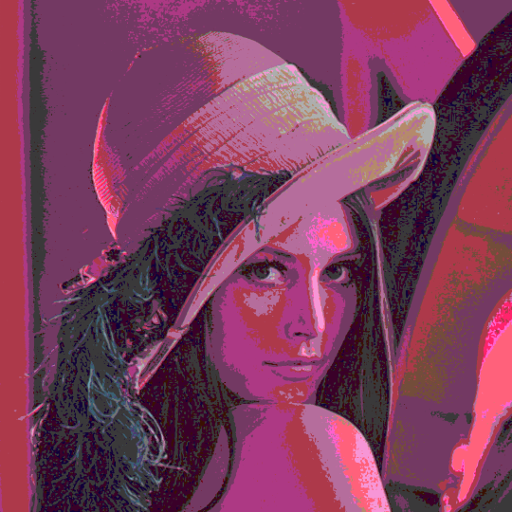
\includegraphics[width=\textwidth]{lena_filter_7}
        \caption{Sedmi filter}
    \end{subfigure}
    \caption{Primerjava originalne slike z obdelano sliko}
    \label{fig:lena_filter_7}
\end{figure}


\subsubsection*{Filter 8}
Osmi filter je sestavljen iz dveh osnovnih filtrov. Najprej sliko obdelamo s
filtrom ``posteriziranje'' in sicer s parametrom $ST = 6$. Rezultat obdelamo
še s filtrom ``uravnovešanje barv'' s parametri $R = -29$, $G = 40$ in $B = 100$.
Rezultat testne slike lahko vidimo na sliki~\ref{fig:lena_filter_8}.

\begin{figure}[!ht]
    \centering
    \begin{subfigure}[b]{0.4\textwidth}
        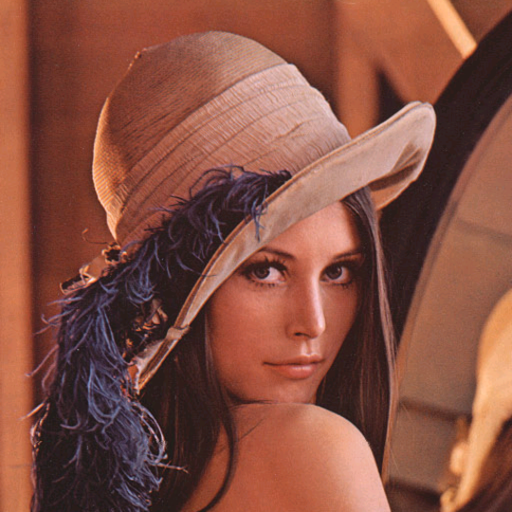
\includegraphics[width=\textwidth]{lena}
        \caption{Original}
    \end{subfigure}
    \begin{subfigure}[b]{0.4\textwidth}
        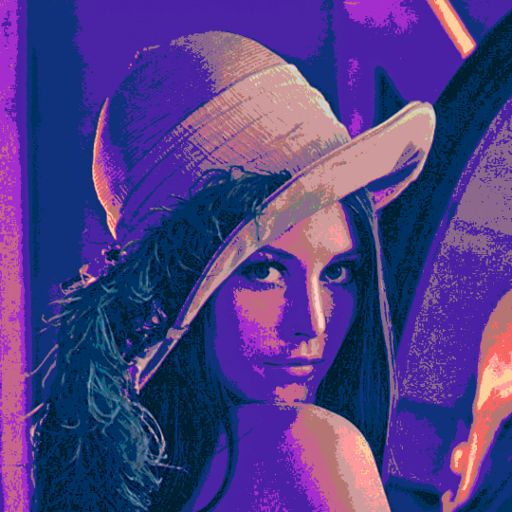
\includegraphics[width=\textwidth]{lena_filter_8}
        \caption{Osmi filter}
    \end{subfigure}
    \caption{Primerjava originalne slike z obdelano sliko}
    \label{fig:lena_filter_8}
\end{figure}


\subsubsection*{Filter 9}
Deveti filter je sestavljen iz dveh osnovnih filtrov. Najprej sliko obdelamo s
filtrom ``uravnovešanje barv v HSL prostoru'' in sicer s parametri $H = -41$,
$L = -20$ in $S = 25$. Rezultat obdelamo še s filtrom ``posteriziranje'' s
parametrom $ST = 4$. Rezultat testne slike lahko vidimo na
sliki~\ref{fig:lena_filter_9}.

\begin{figure}[!ht]
    \centering
    \begin{subfigure}[b]{0.4\textwidth}
        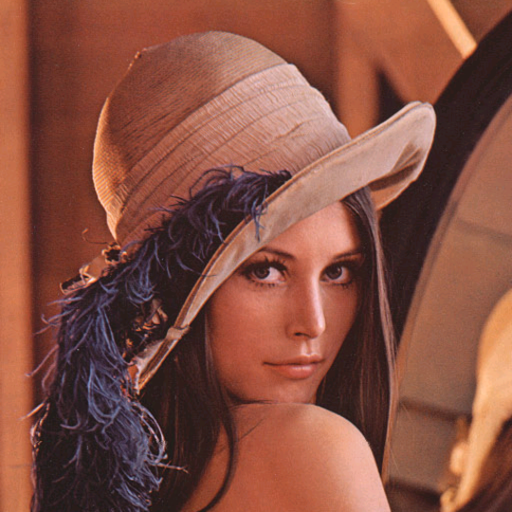
\includegraphics[width=\textwidth]{lena}
        \caption{Original}
    \end{subfigure}
    \begin{subfigure}[b]{0.4\textwidth}
        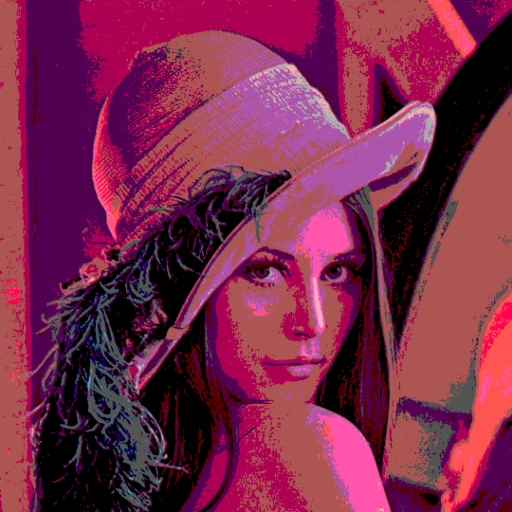
\includegraphics[width=\textwidth]{lena_filter_9}
        \caption{Deveti filter}
    \end{subfigure}
    \caption{Primerjava originalne slike z obdelano sliko}
    \label{fig:lena_filter_9}
\end{figure}


\subsubsection*{Filter 10}
Deseti filter je sestavljen iz treh osnovnih filtrov. Najprej sliko obdelamo s
filtrom ``uravnovešanje barv'' in sicer s parametri $R = 100$, $G = -100$ in
$B = -100$. Rezultat obdelamo še s filtrom ``posteriziranje'' s parametrom
$ST= 3$ in nazadnje še s filtrom ``uravnovešanje barv v HSL prostoru'' s
parametri $H = -41$, $L = -10$ in $S = 20$. Rezultat testne slike lahko
vidimo na sliki~\ref{fig:lena_filter_10}.

\begin{figure}[!ht]
    \centering
    \begin{subfigure}[b]{0.4\textwidth}
        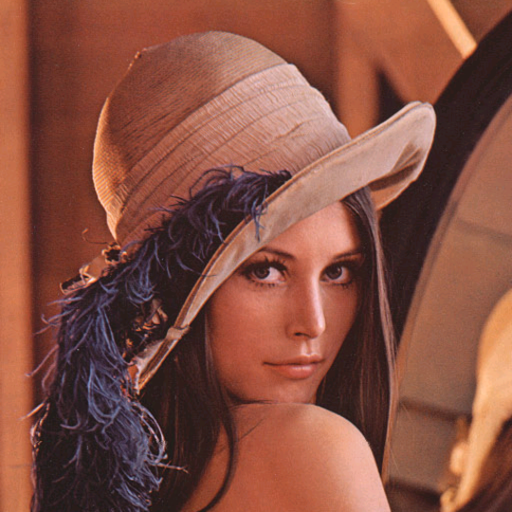
\includegraphics[width=\textwidth]{lena}
        \caption{Original}
    \end{subfigure}
    \begin{subfigure}[b]{0.4\textwidth}
        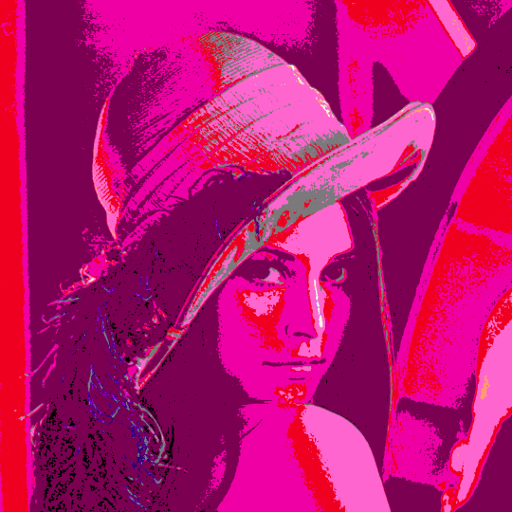
\includegraphics[width=\textwidth]{lena_filter_10}
        \caption{Deseti filter}
    \end{subfigure}
    \caption{Primerjava originalne slike z obdelano sliko}
    \label{fig:lena_filter_10}
\end{figure}


\subsubsection*{Filter 11}
Enajsti filter je sestavljen iz treh osnovnih filtrov. Najprej sliko obdelamo s
filtrom ``uravnovešanje barv'' in sicer s parametri $R = 34$, $G = -38$ in
$B = 24$. Rezultat obdelamo še s filtrom ``posteriziranje'' s parametrom
$ST= 4$ in nazadnje še s filtrom ``uravnovešanje barv v HSL prostoru'' s
parametri $H = -65$, $L = 0$ in $S = 0$. Rezultat testne slike lahko
vidimo na sliki~\ref{fig:lena_filter_11}.

\begin{figure}[!ht]
    \centering
    \begin{subfigure}[b]{0.4\textwidth}
        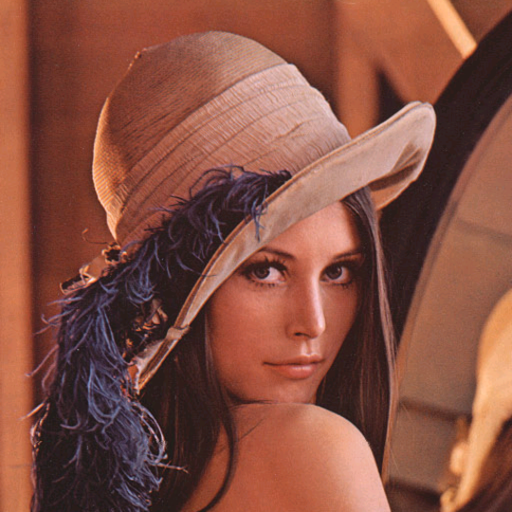
\includegraphics[width=\textwidth]{lena}
        \caption{Original}
    \end{subfigure}
    \begin{subfigure}[b]{0.4\textwidth}
        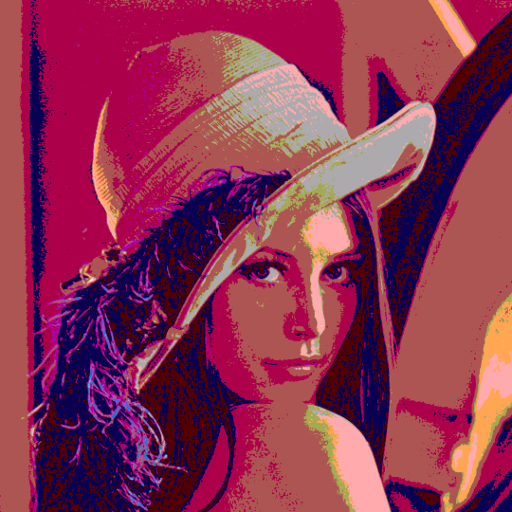
\includegraphics[width=\textwidth]{lena_filter_11}
        \caption{Enajsti filter}
    \end{subfigure}
    \caption{Primerjava originalne slike z obdelano sliko}
    \label{fig:lena_filter_11}
\end{figure}


\subsubsection*{Filter 12}
Dvanajsti filter je sestavljen iz dveh osnovnih filtrov. Najprej sliko obdelamo s
filtrom ``uravnovešanje barv'' in sicer s parametri $R = 40$, $G = -40$ in
$B = 28$. Rezultat obdelamo še s filtrom ``posteriziranje'' s parametrom
$ST= 4$ in nazadnje še enkrat s filtrom ``uravnovešanje barv'' vendar s
parametri $R = -100$, $G = -42$ in $B = 100$. Rezultat testne slike lahko
vidimo na sliki~\ref{fig:lena_filter_12}.

\begin{figure}[!ht]
    \centering
    \begin{subfigure}[b]{0.4\textwidth}
        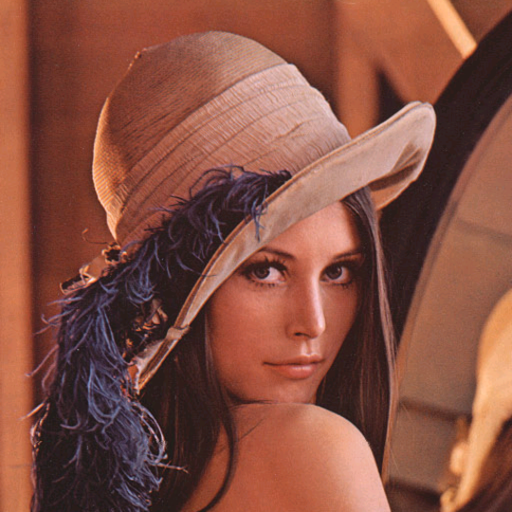
\includegraphics[width=\textwidth]{lena}
        \caption{Original}
    \end{subfigure}
    \begin{subfigure}[b]{0.4\textwidth}
        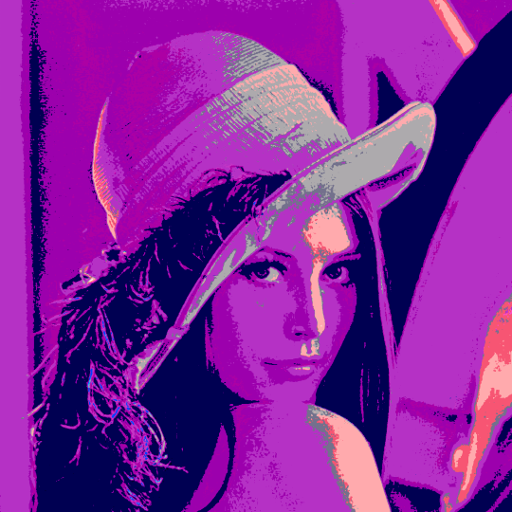
\includegraphics[width=\textwidth]{lena_filter_12}
        \caption{Dvanajsti filter}
    \end{subfigure}
    \caption{Primerjava originalne slike z obdelano sliko}
    \label{fig:lena_filter_12}
\end{figure}


\subsubsection*{Filter 13}
Trinajsti filter je sestavljen iz dveh osnovnih filtrov. Najprej sliko obdelamo s
filtrom ``uravnovešanje barv'' in sicer s parametri $R = 45$, $G = -45$ in
$B = 35$. Rezultat obdelamo še s filtrom ``posteriziranje'' s parametrom
$ST =4$. Rezultat testne slike lahko vidimo na sliki~\ref{fig:lena_filter_13}.

\begin{figure}[!ht]
    \centering
    \begin{subfigure}[b]{0.4\textwidth}
        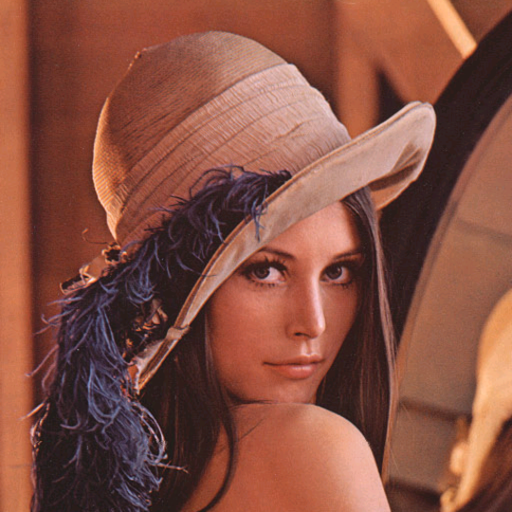
\includegraphics[width=\textwidth]{lena}
        \caption{Original}
    \end{subfigure}
    \begin{subfigure}[b]{0.4\textwidth}
        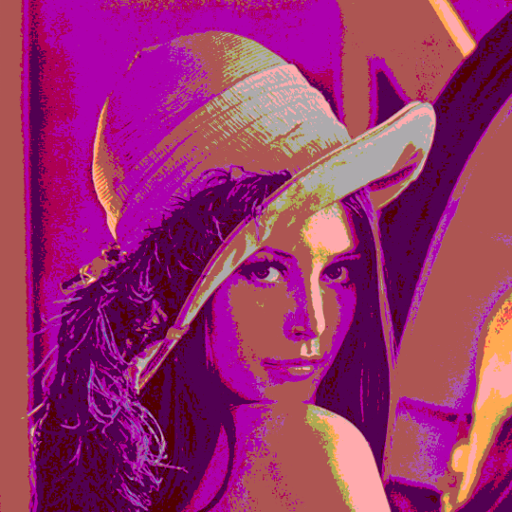
\includegraphics[width=\textwidth]{lena_filter_13}
        \caption{Trinajsti filter}
    \end{subfigure}
    \caption{Primerjava originalne slike z obdelano sliko}
    \label{fig:lena_filter_13}
\end{figure}


\subsubsection*{Filter 14}
Štirinajsti filter je sestavljen iz dveh osnovnih filtrov. Najprej sliko obdelamo s
filtrom ``uravnovešanje barv'' in sicer s parametri $R = -45$, $G = -55$ in
$B = 30$. Rezultat obdelamo še s filtrom ``posteriziranje'' s parametrom
$ST =4$. Rezultat testne slike lahko vidimo na sliki~\ref{fig:lena_filter_14}.

\begin{figure}[!ht]
    \centering
    \begin{subfigure}[b]{0.4\textwidth}
        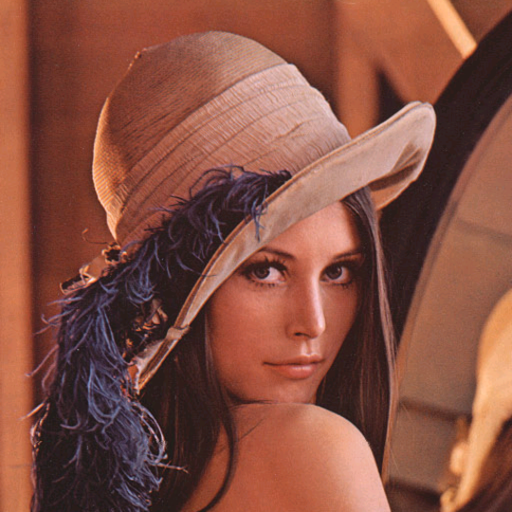
\includegraphics[width=\textwidth]{lena}
        \caption{Original}
    \end{subfigure}
    \begin{subfigure}[b]{0.4\textwidth}
        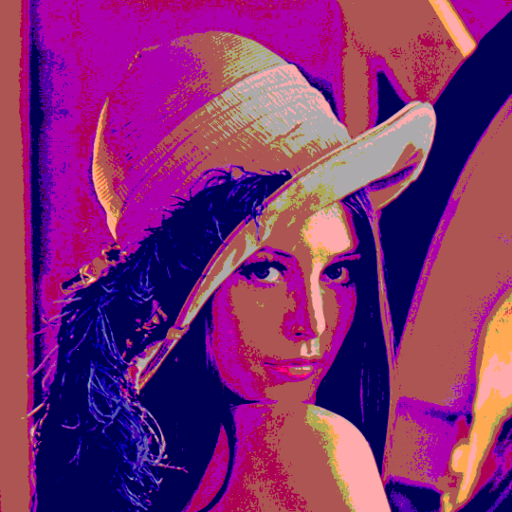
\includegraphics[width=\textwidth]{lena_filter_14}
        \caption{Štirinajsti filter}
    \end{subfigure}
    \caption{Primerjava originalne slike z obdelano sliko}
    \label{fig:lena_filter_14}
\end{figure}


\subsubsection*{Filter 15}
Petnajsti filter vsebuje le osnovni filter ``posteriziranje'' in sicer s parametrom
$ST = 3$. Rezultat testne slike lahko vidimo na sliki~\ref{fig:lena_filter_15}.

\begin{figure}[!ht]
    \centering
    \begin{subfigure}[b]{0.4\textwidth}
        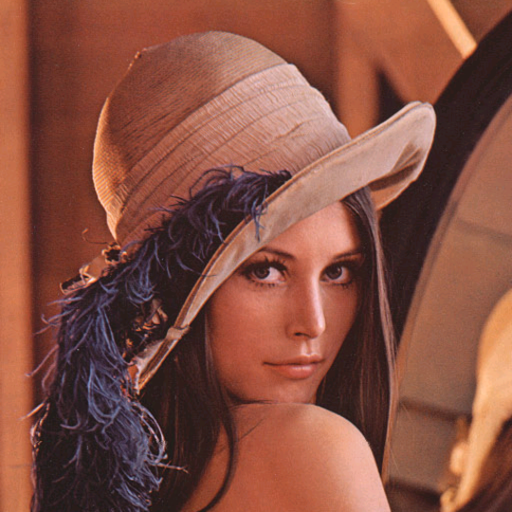
\includegraphics[width=\textwidth]{lena}
        \caption{Original}
    \end{subfigure}
    \begin{subfigure}[b]{0.4\textwidth}
        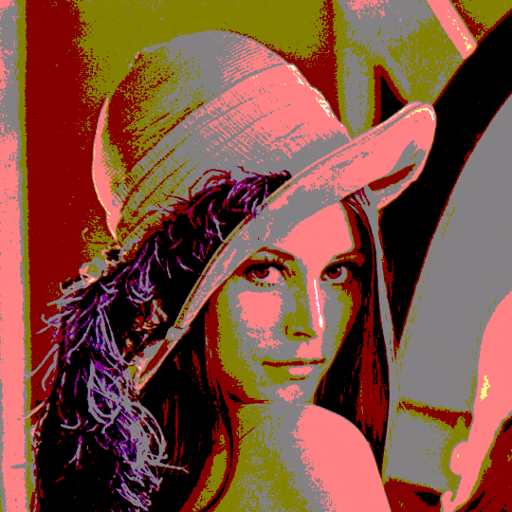
\includegraphics[width=\textwidth]{lena_filter_15}
        \caption{Petnajsti filter}
    \end{subfigure}
    \caption{Primerjava originalne slike z obdelano sliko}
    \label{fig:lena_filter_15}
\end{figure}


\subsubsection*{Filter 16}
Šestnajsti filter je sestavljen iz dveh osnovnih filtrov. Najprej sliko obdelamo s
filtrom ``uravnovešanje barv'' in sicer s parametri $R = 30$, $G = -40$ in
$B = 16$. Rezultat obdelamo še s filtrom ``posteriziranje'' s parametrom
$ST =3$. Rezultat testne slike lahko vidimo na sliki~\ref{fig:lena_filter_16}.

\begin{figure}[!ht]
    \centering
    \begin{subfigure}[b]{0.4\textwidth}
        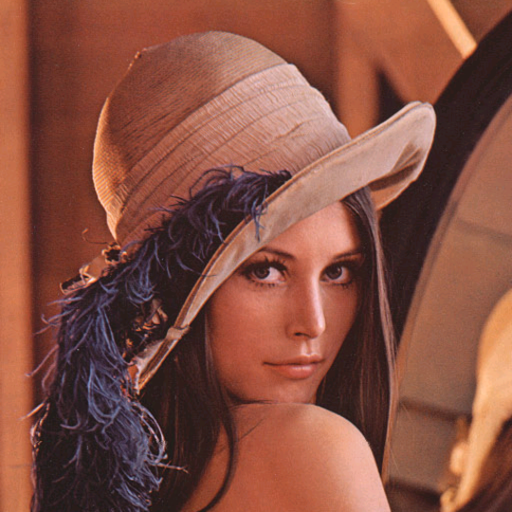
\includegraphics[width=\textwidth]{lena}
        \caption{Original}
    \end{subfigure}
    \begin{subfigure}[b]{0.4\textwidth}
        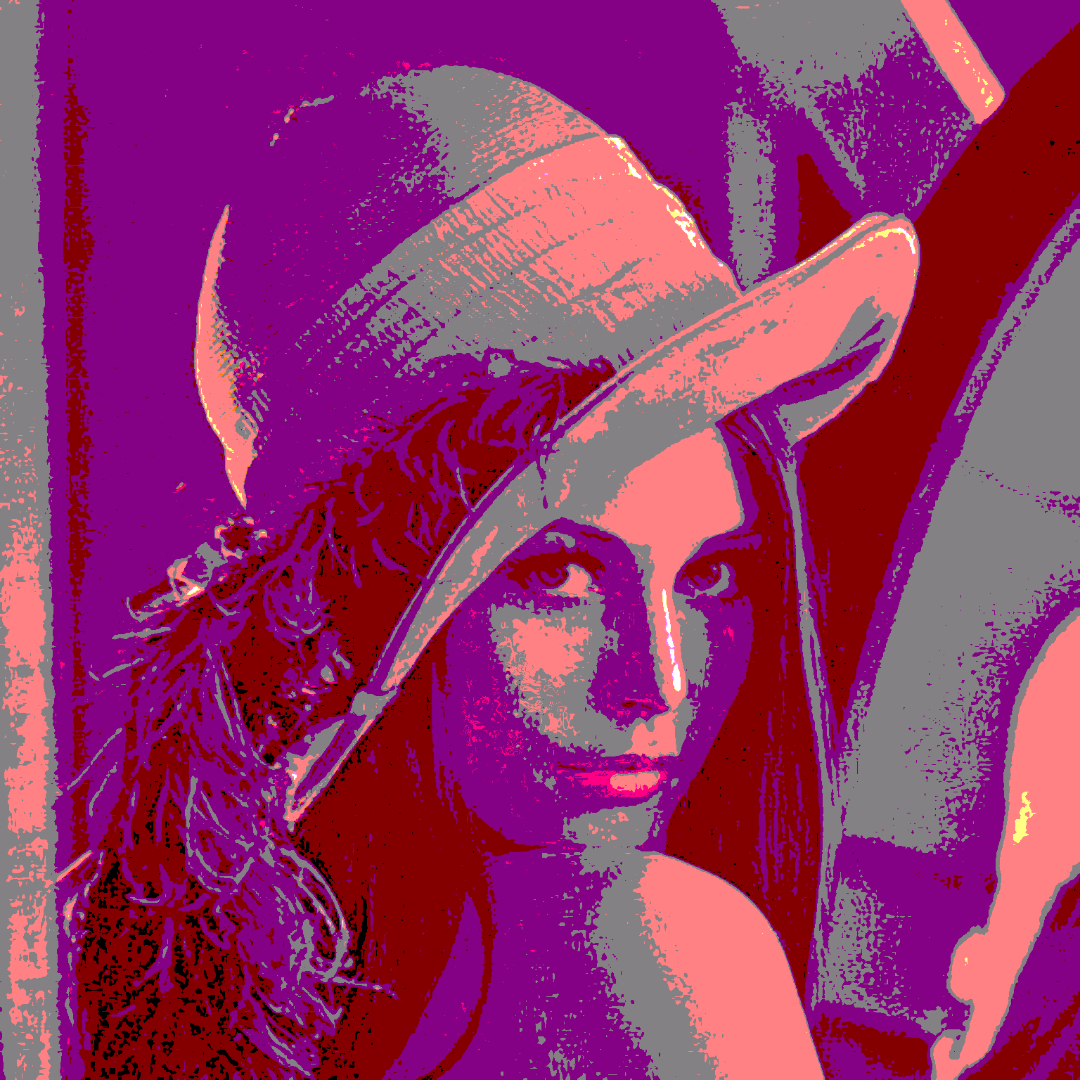
\includegraphics[width=\textwidth]{lena_filter_16}
        \caption{Šestnajsti filter}
    \end{subfigure}
    \caption{Primerjava originalne slike z obdelano sliko}
    \label{fig:lena_filter_16}
\end{figure}


\subsubsection*{Filter 17}
Sedemnajsti filter je sestavljen iz treh osnovnih filtrov. Najprej sliko obdelamo s
filtrom ``uravnovešanje barv'' in sicer s parametri $R = 20$, $G = -30$ in
$B = 20$. Rezultat obdelamo še s filtrom ``posteriziranje'' s parametrom
$ST= 4$ in nazadnje še s filtrom ``uravnovešanje barv v HSL prostoru'' s
parametri $H = -30$, $L = -10$ in $S = 12$. Rezultat testne slike lahko
vidimo na sliki~\ref{fig:lena_filter_17}.

\begin{figure}[!ht]
    \centering
    \begin{subfigure}[b]{0.4\textwidth}
        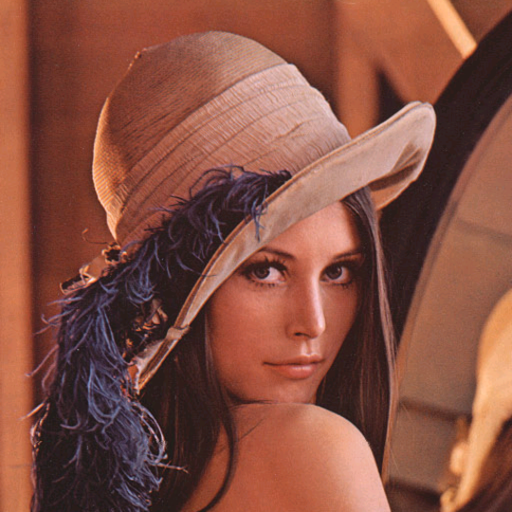
\includegraphics[width=\textwidth]{lena}
        \caption{Original}
    \end{subfigure}
    \begin{subfigure}[b]{0.4\textwidth}
        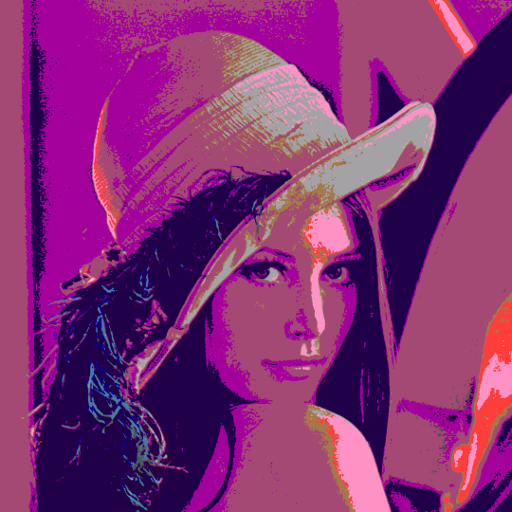
\includegraphics[width=\textwidth]{lena_filter_17}
        \caption{Sedemnajsti filter}
    \end{subfigure}
    \caption{Primerjava originalne slike z obdelano sliko}
    \label{fig:lena_filter_17}
\end{figure}


\chapter{Nove funkcionalne možnosti}
Do sedaj smo originalno instalacijo ``15 sekund slave'' predelovali na način,
da jo ohranjamo kot digitalno umetnost, se pravi brez vidnih sprememb. Vendar
pa kakšna manjša po tako dolgem času lahko le popestri uporabniško izkušnjo.

Najpomembnejša posodobitev, ki bi to umetniško instalacijo naredilo veliko
bolj popularno je integracija s socialnimi omrežji~\ref{ch:social_network}. Dan
danes je to medij, preko katerega se srečamo z veliko ustvarjalnimi idejami.

Naslednja posodobitev, ki prvotno niti ni bila v načrtu, je zamenjava zaslona
LCD. Ta posodobitev se je zgodila zaradi nekompatibilnosti mobilnega telefona
s starim zaslonom LCD. Ko pa je to že bila nujna posodobitev, smo razmišljali
še širše. Večina današnjih zaslonov LCD je formata 16:9 ali pa še več v
širino, starega formata 4:3 skorajda ni več. Naš cilj pa je kvadratna slika.
Najprej smo želeli najti čim bolj kvadraten zaslon. Vendar pa se je kmalu
rodila ideja o še širšem zaslon-u in sicer da je širina malo več kot enkrat
daljša od višine~\ref{fig:frame2}. S tem smo si omogočili možnost prikazovanja
dveh slik. Kot da bi naenkrat imeli razstavljeni dve različici instalacije.
Seveda ima vsaka slika drug obraz, če le ta obstaja.

Zaradi prejšnjega razloga o zamenjavi zaslona je bilo potrebno zamenjati tudi
okvir. Kot že pri prejšnji posodobitvi okvirja bo tudi tokrat ostal bogato
okrašen, le na sredini bo združen, kot je prikazano na sliki~\ref{fig:frame2}.

\begin{figure}[!ht]
    \centering
    \begin{subfigure}[b]{0.33\textwidth}
        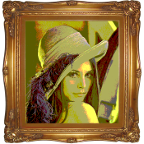
\includegraphics[width=\textwidth]{frame1}
        \caption{Originalni okvir}
    \end{subfigure}
    \begin{subfigure}[b]{0.6\textwidth}
        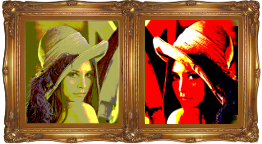
\includegraphics[width=\textwidth]{frame2}
        \caption{Novi razširjeni okvir}
        \label{fig:frame2}
    \end{subfigure}
    \caption{Prikaz razširitve okvirja zaradi menjave širšega zaslona LCD}
\end{figure}


\chapter{Povezovanje s socialnimi omrežji}
\label{ch:social_network}
Ena izmed pomembnejših posodobitev je povezava s socialnimi omrežji, ki so
vsak dan bolj popularna. Vsak dan se na različnih socialnih omrežjih doda na
tisoče žargonsko imenovanih ``selfijev''\footnote{Slika, ko oseba fotografira
samega sebe pri različnih dejavnostih.}. Da pa ta ``selfi'' še bolj pade v
oči, se jim lahko doda kakšen že vnaprej določen filter. Ti so pri pametnih
telefonih, ki so danes ena izmed najpogostejših naprav za fotografiranje
``selfijev'', na voljo samo en dotik stran. Obstajajo pa tudi socialna
omrežja, ki ponujajo osnovne filtre že pri nalaganju slike.

Naša instalacija se lahko interpretira kot generator ``selfijev''. Oseba, ki
stoji pred instalacijo, ve, da bo kmalu njenih petnajst sekund. Pred njo se bo
pokazala pop-art slika, ki je njen umetniški ``selfi'', in če želi, je ta pop-
art slika lahko kmalu javno objavljena na enem izmed socialnih omrežij.


\section{Možnosti}
Najpogosteje so uporabljena naslednja socialna omrežja:
\begin{description}
\item[Facebook]
Trenutno najbolj razširjeno socialno omrežje, ki ga uporabljajo vse
generacije.

\item[Twitter]
Socialno omrežje, najbolj namenjeno kratkim sporočilom imenovanimi ``tviti''.

\item[Instagram]
Socialno omrežje, predvsem namenjeno nalaganju slik. Omogoča tudi veliko
število filtrov za obdelavo le teh.

\item[Google+]
Alternativa socialnemu omrežju Facebook podjetja Google.

\item[Pinterest]
Socialno omrežje, predvsem namenjeno ustvarjalnostim, ki so prikazane v obliki
slik.
\end{description}


\section{Omejitve}
Ena izmed največjih omejitev je nenadzorovano pošiljanje slik na socialno
omrežje. Na slikah so lahko osebe, ki si ne želijo biti objavljene na
socialnem omrežju, saj je javno. Še več, na slikah so lahko otroci, katerih
objavljanje slik na socialnem omrežju je brez dovoljenja staršev prepovedano.
Res je, da smo želeli slike izbrisati petnajst sekund po objavi, vendar pa
večina socialnih omrežjih te slike še vedno hrani, čeprav jih ne vidimo več.
In če se podamo še v najhujšo skrajnost, nekdo bi lahko napisal program, ki
vse slike shranjuje na nek strežnik in nato z njimi razpolagal po svoji volji.


% \chapter{TODO}
% Datoteka {\tt magistrska\_naloga.tex} na kratko opisuje, kako se pisanja
% magistrskega dela lotimo z uporabo programskega pateka \LaTeX. V tem dokumentu
% bomo predstavili nekaj njegovih prednosti in hib. Kar se slednjih tiče, mi
% pride na misel ena sama. Ko se srečamo z njim, nam izgleda kot kislo jabolko,
% nismo prepričani, da bi želeli vanj ugrizniti. Lahko pa z njim pripravimo
% odličen zavitek ali pa pridemo na okus.

% Česa od tega dokumenta ne pričakujte? Izkušeni uporabniki \LaTeX{}a bi vse
% skupaj zastavili drugače. Morda bi napisali posebno razredno datoteko
% (\emph{class file}) --- v resnici priredili katero od obstoječih ---, v
% datoteki {\tt magistrska\_naloga.tex} ohranili samo najbolj grobo strukturo in
% vanjo vključevali  posamezna po\-glav\-ja. Hkrati s pisanjem teksta bi
% poskrbeli tudi za stvarno kazalo ({\tt makeindex}), literaturo pa bi citirali
% z uporabo {\BibTeX}{a}. Tega, skratka, v tem dokumentu ne boste našli.

% Kaj vseeno najdemo. V Poglavju~\ref{ch1} bomo na hitro spoznali besedilne
% konstrukte kot so izreki, enačbe in dokazi. Naučili se bomo, kako se na njih
% sklicujemo. Poglavje~\ref{ch2} bo predstavilo vključevanje plovk: slik in
% tabel. V Poglavju~\ref{ch3} se bomo srečali s sklicevanjem na literaturo.
% Sledil bo samo še zaključek.

% \chapter{Sklicevanje na besedilne konstrukte}
% \label{ch1}
% Matematična ali popolna indukcija je eno prvih orodij, ki jih spoznamo za dokazovanje trditev pri matematičnih predmetih.
% \begin{izrek}
% \label{iz:1}
% Za vsako naravno število $n$ velja
% \begin{equation}
% n < 2^n.
% \label{eq:1}
% \end{equation}
% \end{izrek}
% \begin{dokaz}
% Dokazovanje z indukcijo zahteva, da neenakost~\eqref{eq:1} najprej preverimo za najmanjše naravno število --- $0$. Res, ker je $0 < 1 = 2^0$, je neenačba~\eqref{eq:1} za $n=0$ izpolnjena.

% Sledi indukcijski korak. S predpostavko, da je neenakost~\eqref{eq:1} veljavna pri nekem naravnem številu $n$, je potrebno pokazati, da je ista neenakost v veljavi tudi pri njegovem nasledniku --- naravnem številu $n+1$. Računajmo.
% \begin{align}
% n+1 &< 2^n + 1  \label{eq:2}\\
%     &\le 2^n + 2^n \label{eq:3}\\
%     &= 2^{n+1} \nonumber
% \end{align}
% Neenakost~\eqref{eq:2} je posledica indukcijske predpostavke, neenakost~\eqref{eq:3} pa enostavno dejstvo, da je za vsako naravno število $n$ izraz $2^n$ vsaj tako velik kot 1. S tem je dokaz Izreka~\ref{iz:1} zaključen.
% \end{dokaz}

% Opazimo, da je \LaTeX\ številko izreka podredil številki poglavja.


% \chapter{Plovke: slike in tabele}
% \label{ch2}
% Slike in daljše tabele praviloma vključujemo v dokument kot plovke. Pozicija plovke v končnem izdelku ni pogojena s tekom besedila, temveč z izgledom strani. \LaTeX\ bo skušal plovko postaviti samostojno, praviloma na vrh strani, na kateri se na takšno plovko prvič sklicujemo. Pri tem pa bo na vsako stran končnega izdelka želel postaviti tudi sorazmerno velik del besedila. V skrajnem primeru, če imamo res preveč plovk, se bo odločil za stran popolnoma zapolnjeno s plovkami.

% \section{Formati slik}
% Bitne slike, vektorske slike, kakršnekoli slike, z \LaTeX{}om lahko vključimo vse.
% Slika~\ref{pic1} je v {\tt .pdf} formatu.
% \begin{figure}
%     \begin{center}
%         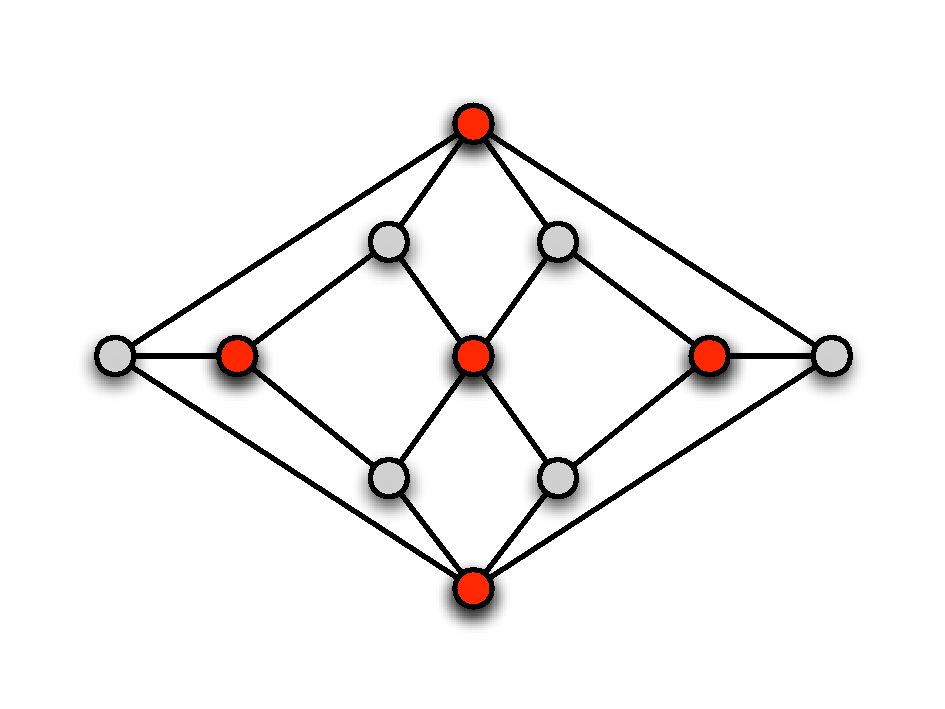
\includegraphics[width=10cm]{pic1.pdf}
%     \end{center}
% \caption{Herschelov graf, vektorska grafika.}
% \label{pic1}
% \end{figure}
% Pa res lahko vključimo slike katerihkoli formatov? Žal ne. Programski paket \LaTeX\ lahko uporabljamo v več dialektih. Ukaz {\tt latex} ne mara vključenih slik v formatu Portable Document Format {\tt .pdf}, ukaz {\tt pdflatex} pa ne prebavi slik v Encapsulated Postscript Formatu {\tt .eps}.
% Strnjeno v Tabeli~\ref{tbl:1}.

% \begin{table}
%     \begin{center}
%         \begin{tabular}{l|ccc}
%             ukaz/format & {\tt .pdf} & {\tt .eps} & ostali formati \\ \hline
%                         {\tt pdflatex} & da & ne & da \\
%                         {\tt latex}   & ne & da  & da
%         \end{tabular}
%     \end{center}
% \caption{}
% \label{tbl:1}
% \end{table}

% Nasvet? Odločite se za uporabo ukaza {\tt pdflatex}. Vaš izdelek bo brez vmesnih stopenj na voljo v {.pdf} formatu in ga lahko odnesete v vsako tiskarno. Če morate na vsak način vključiti sliko, ki jo imate v {\tt .eps} formatu, jo vnaprej pretvorite v alternativni format, denimo {\tt .pdf}.

% Včasih se da v okolju za uporabo programskega paketa \LaTeX\ nastaviti na kakšen način bomo prebavljali vhodne dokumente. Spustni meni na Sliki~\ref{pic2} odkriva uporabo \LaTeX{}a v njegovi pdf inkarnaciji --- {\tt pdflatex}.
% \begin{figure}
% \begin{center}
% 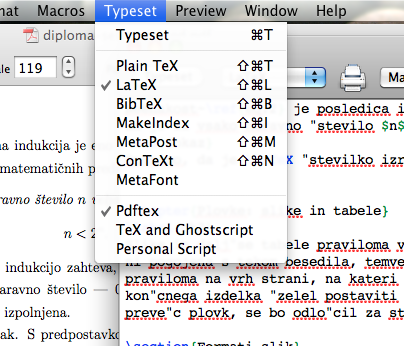
\includegraphics[width=10cm]{pic2.png}
% \end{center}
% \caption{Kateri dialekt uporabljati?}
% \label{pic2}
% \end{figure}

% Vključena Slika~\ref{pic2} je seveda bitna.

% Kaj pa stran iz študentskega referata?\label{pp}
% Tudi njo lahko vključimo v dokument. Toda ne kot plovko.


% \chapter{Kaj pa literatura?}
% \label{ch3}
% Kot smo omenili že v uvodu, je pravi način za citiranje literature uporaba \BibTeX{}a~\cite{bib}.
% Programski paket \LaTeX je prvotno predstavljen v priročniku~\cite{lat} in je v resnici nadgradnja sistema \TeX\ avtorja Donalda Knutha, znanega po denimo, če izpustim njegovo umetnost programiranja, Knuth-Bendixovem algoritmu~\cite{dk1}.

% Vsem raziskovalcem s področja računalništva pa svetujem v branje mnenje L.\ Fortnowa~\cite{lf}~\cite{trifonova}.

\chapter{Sklepne ugotovitve}
Izbira \LaTeX\ ali ne \LaTeX\ je seveda prepuščena vam samim. Res je, da so
prvi koraki v \LaTeX{}u težavni. Ta dokument naj vam služi kot začetna opora
pri hoji.
